\documentclass[pdflatex,11pt]{aghdpl}
%\documentclass[pdflatex,11pt,openright,b5paper]{pl_book}
% \documentclass{aghdpl}               % przy kompilacji programem latex
% \documentclass[pdflatex,en]{aghdpl}  % praca w~języku angielskim
\usepackage{hyphenat}
\usepackage[T1]{fontenc}
\usepackage{natbib}
\usepackage[polish]{babel}
\usepackage[utf8]{inputenc}
\usepackage{wrapfig}
\usepackage{graphicx}
\usepackage{subcaption}
\usepackage[font={small}]{caption}
\usepackage{float}
\usepackage{amsmath}
\usepackage{amsfonts}
\usepackage[outercaption]{sidecap}    

\usepackage{titlesec}
\titleclass{\chapter}{top}

\setcitestyle{square}


\usepackage{nomencl}
\makenomenclature

% dodatkowe pakiety
\usepackage{enumerate}
\usepackage{listings}
\lstloadlanguages{TeX}

\lstset{
  literate={ą}{{\k{a}}}1
           {ć}{{\'c}}1
           {ę}{{\k{e}}}1
           {ó}{{\'o}}1
           {ń}{{\'n}}1
           {ł}{{\l{}}}1
           {ś}{{\'s}}1
           {ź}{{\'z}}1
           {ż}{{\.z}}1
           {Ą}{{\k{A}}}1
           {Ć}{{\'C}}1
           {Ę}{{\k{E}}}1
           {Ó}{{\'O}}1
           {Ń}{{\'N}}1
           {Ł}{{\L{}}}1
           {Ś}{{\'S}}1
           {Ź}{{\'Z}}1
           {Ż}{{\.Z}}1
}

%---------------------------------------------------------------------------

\author{Marcin Stolarek}
\shortauthor{M. Stolarek}

%\titlePL{Elementy dyfrakcyjne, refracyjne i~absorpcyjne oparte na podfalowych periodycznych strukturach metalicznych}
\titlePL{Elementy dyfrakcyjne, refrakcyjne i~absorpcyjne oparte na podfalowych periodycznych strukturach metalicznych}
\titleEN{Diffractive, refractive and absorptive optical elements based on periodic sub-wavelength metallic structures}

%\shorttitle{Elementy dyfrakcyjne, refracyjne i~absorpcyjne oparte na podfalowych periodycznych strukturach metalicznych} % skrócona wersja tytułu jeśli jest bardzo długi
\shorttitlePL{Elementy dyfrakcyjne, refrakcyjne i~absorpcyjne oparte na podfalowych periodycznych strukturach metalicznych} % skrócona wersja tytułu jeśli jest bardzo długi
\shorttitleEN{Diffractive, refractive and absorptive optical elements based on periodic sub-wavelength metallic structures}

%\thesistype{Rozprawa doktorska}
\thesistypePL{Rozprawa doktorska}
\thesistypeEN{Phd in physics}

%\supervisor{dr hab. Rafał Kotyński}
\supervisorPL{dr hab. Rafał Kotyński}
\supervisorEN{Rafał Kotyński Ph.D}

\date{2016}

\departmentPL{Zakład Optyki Informacyjnej}
\departmentEN{Information Optics Department}

\facultyPL{Wydział Fizyki}
\facultyEN{Faculty of Physics}

\acknowledgements{Serdecznie dziękuję \dots }



\setlength{\cftsecnumwidth}{10mm}

%---------------------------------------------------------------------------

\begin{document}
\frontmatter

\titlepages

\tableofcontents
\clearpage

\mainmatter

\chapter{Wstęp}
\section{Wprowadzenie}
Optyka jest częścią fizyki, która po szkolnym kursie kojarzy się większości z~wyznaczaniem biegu promieni świetlnych zgodnie z~zasadami optyki geometrycznej. Podstawowe elementy, z~których budowane są zadania do rozwiązania przez uczniów to soczewki i~pryzmaty, tworzące niezbyt skomplikowany, w~porównaniu z~innymi, dział fizyki. Powstaje wrażenie, że w~nauce o~świetle nie ma miejsca na niespodzianki, nowe odkrycia czy nawet zaskakujące wykorzystanie znanych praw. Zgłębianie zagadnień związanych z~elektromagnetyzmem, prowadzi nas jednak w~świat, w~którym dokonuje się wielu zaskakujących odkryć poszerzających nasze zrozumienie i~umożliwiających różnorakie zastosowania.

Skupiając się na ostatnich trzydziestu latach historii optyki dostrzec możemy wiele kroków milowych dokonanych przez fizyków na całym świecie. Z pewnością jednym z~najbardziej istotnych był opis kryształów fotonicznych, w~których struktura geometryczna narzuca ograniczenia na ruch fotonów na zasadach analogicznych do wpływu jaki wywiera sieć krystaliczna w~ciałach stałych na poruszające się w~nich elektrony. Chociaż tego rodzaju struktury były badane przez ludzi jeszcze w~XIX wieku, to sam termin jak i~nowatorskie podejście znajdujące głęboką analogię do fizyki półprzewodników pojawiły się dopiero po kluczowych pracach Eli Yablonovitscha~\cite{yablonovitch1987inhibited} i~Sajeeva Johna~\cite{john1987strong}. W szczególności przytoczeni autorzy zauważyli możliwość występowania fotonicznej przerwy wzbronionej.

Znaczący wpływ na postrzeganie elektromagnetyzmu miało wprowadzenie ,,optyki transformacyjnej'', której podwaliny stworzyli Ward i~Pendry~\cite{ward1996refraction}. Zaproponowane  przez nich podejście do równań Maxwella polegające na równoważnym potraktowaniu transformacji przestrzeni i~przenikalności elektrycznej i~magnetycznej jest analogiczne do zakrzywienia przestrzeni przez grawitację w~ogólnej teorii względności. Najbardziej spektakularnym przewidywaniem teoretycznym, opartym na optyce transformacyjnej, które zostało również potwierdzone w~eksperymentach jest płaszcz niewidzialności~\cite{schurig2006metamaterial}.

Jedynym z~najbardziej podstawowych zastosowań optyki przez stulecia było obrazowanie, czyli tworzenie obrazu rzeczywistego obiektu w~innym miejscu w~przestrzeni niż znajduje się obiekt. Zastosowanie znajdują tu zazwyczaj soczewki, nieodłącznym w~dziejach ludzkości elementem optycznym wykorzystującym naturalną soczewkę, do obrazowania właśnie, jest ludzkie oko. Ewentualne wady ludzkiej soczewki mogą być korygowane przy pomocy dodatkowych soczewek w~postaci okularów czy szkieł kontaktowych. Zapewne z tego względu wielu moich znajomych w~trakcie studiów, gdy mówiłem, że zajmuję się optyką kojarzyło mnie z~kimś zajmującym się okularami.

Tradycyjne soczewki posiadają jednak znaczące ograniczenie (oczywiście nieistotne w~kontekście konstrukcji okularów do korekcji widzenia). Przy ich pomocy nie jest możliwe skupianie światła w~obszarach znacznie mniejszych od połowy długości fali. Pierwsza propozycja teoretyczna stworzenia idealnej soczewki została podana przez Pendry'ego \cite{PhysRevLett.85.3966}, a oparta była na wykorzystaniu materiałów o ujemnej przenikalności elektrycznej, których własności teoretycznie analizował już w~latach sześćdziesiątych XX wieku Wiesiełago \cite{veselago1968electrodynamics}. Dalsze prace dotyczące supersoczewek czy hipersoczewek \cite{liu2007far} znacznie poszerzyły potencjalne zastosowania światła widzialnego w~obszarach takich jak obrazowanie czy litografia wysokorozdzielcza wykorzystująca światło widzialne. Obrazowaniu nadrozdzielczemu poświęcony jest rozdział \ref{art:nondiff}.

Innym odkryciem dla którego kluczowe znaczenia ma występowanie powierzchniowych plazmonów polarytonów jest nadzwyczajna transmisja fal elektro-magnetycznych przez szczeliny o rozmiarach podfalowych. Analiza tego zjawiska została przedstawiona w~1998 przez Ebbesena i~innych \cite{ebbesen1998extraordinary}. Prace te stanowią podstawę dla analizowanych w~rozdziale \ref{chap:thz} niniejszej rozprawy podfalowych siatek dyfrakcyjnych wykazujących transmisję asymetryczną.

Poniższa praca jest kolejnym, małym wkładem, czynionym prez tysiące fizyków na całym świecie służącym pogłębienu wiedzy o~świecie, w~szczgólności o~zjawiskach optycznych i~umożliweniu jej zastosowania.

\section{Cele i~tezy pracy}
Głównymi zadaniami realizowanymi przez autora było wykorzystanie metod obliczeniowych w~celu projektowania i~optymalizacji struktury podfalowych do kształtowania fal elektromagnetycznych. Rozważania dotyczyły zarówno zakresu widzialnego i~dalekiej podczerwieni, aż po symulacje dotyczące fal E-M o~częstotliwościach terahercowych. W wyniku przeprowadzonych prac sformułowane zostały następujące tezy, dotyczące zarówno aspektów teoretycznych jak i~posiadających kontekst eksperymentalny:
\begin{itemize}

\item Podwójne siatki metalowe, jako układy liniowe, zgodne z~twierdzeniem o~wzajemności Lorenza nie mogą posłużyć do konstrukcji izolatorów optycznych. Asymetria w~kierunku transmisji w~odpowiednio zaprojektowanych strukturach DMG osiągana jest w~-1~i~+1 rzędzie dyfrakcyjnym, dzięki czemu omawiane struktury mogą zostać wykorzystane w~geometrii cylindrycznej do konstrukcji soczewek dyfrakcyjnych.

\item Możliwe jest wykorzystanie metalowych siatek dyfrakcyjnych w~celu budowy wąskopasmowych, efektywnych anten promieniowania THz opartego na tranzystorach polowych realizowanych w~podkładzie z~półprzewodników. 

\item Możliwa jest eksperymentalna realizacja metamateriału absorpcyjnego o~własnościach podobnych do PML dla długości fali z~zakresu podczerwieni. Tego typu absorbery choć złożone z~warstw o~rozmiarach podfalowych, same osiągają jednak grubości zbliżone do długości fali lub większe gdy wymagane jest osiągnięcie niskiego współczynnika odbicia dla padania pod kątami bliskimi $90^{\circ}$.

\item Realizacja metamateriałów charakteryzujących się propagacją światła nie podlegającą ograniczeniu dyfrakcyjnemu opartych o~wielowarstwy metaliczno-dielektryczne wymaga możliwości bardzo gładkiego napylania warstw. Chropowatości charakteryzujące się $RMS>1$~nm mogą uniemożliwić praktyczne wykorzystanie takich struktur, szczególnie w~przypadku stosów zawierających znaczną liczbę (ok 10) warstw.
\end{itemize}

\section{Podział pracy}
Niniejsza rozprawa doktorska składa się ze wstępu, pięciu rozdziałów zasadniczych oraz rozdziału szóstego, stanowiącego podsumowanie pracy. Wstęp zawiera niezbędne elementy wprowadzające w tematykę kształtowania fal elektromagnetycznych oraz przedstawia tezy rozprawy doktorskiej. Rozdział drugi stanowi wprowadzenie do metod modelowania elektromagnetycznego. Opisane w~nim zostały stosowane w~symulacjach metody numeryczne, szczególnie dokładnie metoda różnic skończonych w~dziedzinie czasu (ang. FDTD finite-difference time-domain). Rozdział ten zawiera również podstawy teorii układów liniowych niezmienniczych ze względu na przesunięcia wraz z~elementami optyki fourierowskiej. Zawiera także wstęp do przybliżenia ośrodka efektywnego stosowanego dla wielowarstw, o których mowa w~rozdziale czwartym i~piątym.

Rozdział trzeci poświęcony jest projektowaniu układów przeznaczonych dla zakresu terahercowego. Rozdział traktuje o możliwości wykorzystania metalowych siatek dyfrakcyjnych w~roli anten promieniowania terahercowego. Wskazane zostały możliwości transmisji  selektywnej - rezonansowej. Zachodzące zjawiska przedstawiono w~sposób jakościowy, opierając się na współczesnej literaturę przedmiotu. Dokładny opis ilościowy opiera się na obliczeniach autora pracy, pozwalających na dokładne określenie granic stosowalności przybliżeń teoretycznych w~zakresie modelowania własności materiałów i~samych siatek dyfrakcyjnych. W dalszej części rozdziału przedstawione zostały struktury określane w~literaturze mianem podwójnych siatek metalowych. Opisany został wpływ odpowiednich parametrów geometrycznych DMG~(ang. double metallic grating) na współczynniki transmisji. Przedstawiono możliwości uzyskania transmisji asymetrycznej wraz z~zaprzeczeniem funkcjonowania omawianych układów w~charakterze diody optycznej. Zakończenie rozdziału stanowi omówienie możliwości wykorzystania DMG w~geometrii cylindrycznej jako jednokierunkowej soczewki promieniowania THz.

Rozdziały czwarty i~piąty poświęcone są metamateriałom o budowie opartej na strukturach warstwowych. Rozdział czwarty zaczyna się krótkim wprowadzeniem do tematyki warstw nieodbijających. Przedstawiona zostaje zarówno klasyczna warstwa antyodbiciowa, jak i nowsze rozwiązania pojawiające się w literaturze w ostatnich latach. W dalszej części wyprowadzony zostaje oparty na~zasadach optyki transformacyjnej nieodbijający ośrodek pochłaniający promieniowanie E-M, w~obliczeniach numerycznych określany jako PML~(od ang. perfectly matched layer). Omówiona zostaje możliwość realizacji metamateriału absorpcyjnego o~charakterystyce PML za pomocą wielowarstwy, w~granicy homogenizacji opisywanej efektywnymi tensorami przenikalności elektrycznej i~magnetycznej odpowiadającymi wybranemu PML. Dyskusji poddana zostaje możliwość realizacji metamateriału za pomocą substancji występujących w~przyrodzie, nieposiadających zysku optycznego oraz własności magnetycznych w~zakresach światła widzialnego i~podczerwieni. Ostatecznie przedstawione są wyniki eksperymentów numerycznych dla metamateriału o~własnościach podobnych do PML składającego się z~rzeczywistych substancji.

W kolejnym rozdziale omówione zostały wielowarstwy metaliczno-dielektryczne umożliwiające propagację światła niepodlegającą klasycznemu ograniczeniu dyfrakcyjnemu. W pierwszych częściach rozdziału czytelnik może się zapoznać ze współczesnym stanem wiedzy w~dziedzinie obrazowania podfalowego. W dalszej części rozdziału - na podstawie wyników obliczeniowych autora pracy oraz informacji literaturowych - omówione zostały możliwości budowy bardziej skomplikowanych elementów optycznych pozwalających na uzyskanie podfalowej koncentracji światła oraz na realizację operacji geometrycznych rzutowania, obrotu na podfalowych rozkładach pola elektromagnetycznego. Analizie numerycznej poddane są w szczególności wielowarstwy chropowate o topologii odpowiadającej warstwom powstającym przy napylaniu metodą fizycznego osadzania z fazy gazowej (ang.~physical vapour deposition~-~PVD). Przedyskutowany zostaje wpływ niedoskonałości warstw na właściwości obrazujące i transmisyjne metamateriałów. Na podstawie własnych wyników numerycznych oraz pracach innych autorów sformułowane zostają wymogi dotyczące gładkości napylenia warstw.

Ostatni rozdział stanowi podsumowanie rozprawy. Wskazano w nim kluczowe wnioski i podano argumentację tez rozprawy wraz z odniesieniem do treści pracy.













\section{Metody numeryczne}
\subsection{Metody  macierzowe}
\subsection{FDTD}
\label{subart:fdtd}
Metoda różnic skończonych w~dziedzinie czasu (ang. FDTD - finite-difference time-domain) jest szeroko wykorzystywana w~niniejszej pracy ze względu na możliwości symulowania ośrodków materialnych opisywanych modelem Lorenza-Drudego \ref{subart:lorenz-drude}, oraz bezpośrednie obliczanie wartości pól $E$ i~$H$ we wszystkich punktach siatki obliczeniowej. Poniżej przedstawione zostały podstawowe elementy tej metody symulacji numerycznych. Podstawą do współcześnie prowadzonych symulacji elektromagnetycznych w~dziedzinie czasu jest algorytm różnic skończonych z~krokiem skokowym~(ang. leapfrog)  odnoszący się do dyskretyzacji przestrzeni i~czasu w~komórce dyskretyzacji Yee~\cite{1966ITAP14302Y}, który rozwiązywanie równań Maxwella sprowadza do następującej sekwencji:
\begin{enumerate}
\item Zastąpienie wszystkich pochodnych cząstkowych w~prawach Amp\`{e}r'a i~Faradaya różnicami skończonymi.
\item Przekształcenie powstałych równań, tak aby wyrazić amplitudy pól $E$ i~$H$ w~czasie $t_0 +  \Delta_t$ przez ich wartości w~czasie $t_0$, oraz wartości drugiego pola w~czasie $t_0+ \frac{\Delta_t}{2}$.
\item Obliczenie wartości pola $H$ w~czasie $t_0 +  \Delta_t$.
\item Obliczenie na podstawie wartości $H$ dla $t=t_0+  \Delta_t$, wartości pola $E$ w~czasie $t_0 + \frac{3}{2} \Delta_t$.
\item Powtarzanie kroków 3-4 w celu ewolucji stanu układu przez żądany czas.
\end{enumerate}
Działanie algorytmu Yee zostanie teraz przedstawione bardziej szczegółowo na przykładzie, który pozwoli lepiej prześledzić powyższe skrótowo opisane kroki. Ponieważ prowadzenie rachunków dla problemu trójwymiarowego byłoby przesadnie skomplikowane, dla celów poglądowych skupimy się na zagadnieniu jednowymiarowym.

Załóżmy, że pole elektryczne jest spolaryzowane w~kierunku $z$, w~jednowymiarowej przestrzeni opisywanej przez oś x ($\vec{E}=E_z \cdot \hat{e_z}$). W takiej sytuacji prawo Faradaya możemy zapisać jako:
\begin{equation}
\mu \frac{\partial \vec{H}}{\partial t}= \mu \frac{\partial H_y}{\partial t} \hat{e_y}= \nabla \times \vec{E} = - \frac{\partial E_z}{\partial x} \hat{e_y} 
\label{eq:fdtd-faraday}
\end{equation}
Zgodnie z~oczekiwaniami jedyną zmienną w~czasie składową natężenia pola magnetycznego jest $H_y$. Wykorzystując ten fakt możemy również uprościć zapis prawa Amp\`{e}r'a:
\begin{equation}
\varepsilon \frac{\partial \vec{E}}{\partial t}=\nabla \times \vec{H} = \frac{\partial H_y}{\partial x} \hat{e_z}
\label{eq:fdtd-amper}
\end{equation}
Z powyższych równań możemy wyznaczyć skalarny układ równań różniczkowych na składowe $H_y$ i~$E_z$,
\begin{equation}
\mu \frac{\partial H_y}{\partial t}=\frac{\partial E_z}{\partial x} ,
\varepsilon \frac{\partial E_z}{\partial t}=\frac{\partial H_y}{\partial x},
\end{equation} w~którym zmiana w~czasie amplitudy jednego z~pól wyrażona jest przez pochodną względem $x$ drugiego pola. Równanie wyprowadzone z~(\ref{eq:fdtd-faraday}) posłuży nam do wyznaczenia zmiany w~czasie natężenia pola magnetycznego, natomiast równanie~(\ref{eq:fdtd-amper}) do obliczenia przyszłych (w czasie $t_0 + \Delta_t$) wartości pola $E$.

\begin{figure}[tb]
\includegraphics[width=.9\textwidth]{subart/fdtd/leapfrog.png}
\caption{Graficzna prezentacja dyskretyzacji w~jednowymiarowej metodzie FDTD. Pozioma przerywana linia wskazuje przykładową granicę pomiędzy wartościami już obliczonymi i~szukanymi w~kolejnym kroku symulacji. }
\label{pic:leapfrog}
\end{figure}

 Wprowadzając konwencję przypisywania górnych indeksów $q$  iteracjom algorytmu oraz umieszczanych w~nawiasach kwadratowych indeksów $m$ opisujących położenie w~przestrzeni, możemy wyprowadzić formuły na wartości obu pól
\begin{equation}
H_y^{q+\frac{1}{2}}[m+\frac{1}{2}]=H_y^{q-\frac{1}{2}}+\frac{\Delta_t}{\mu \Delta_x}(E^q_z[m+1]-E^q_z[m]),
\label{eq:numhy-1dfdtd}
\end{equation}

\begin{equation}
E_z^{q+1}[m]=E_z^{q}+\frac{\Delta_t}{\varepsilon \Delta_x}(H^{q+\frac{1}{2}}_z[m+\frac{1}{2}]-H^{q-\frac{1}{2}}_z[m-\frac{1}{2}]),
\label{eq:numez-1dfdtd}
\end{equation}
 Ponieważ wartości tych pól w~kolejnym kroku czasowym wyrażane są jedynie przez wartość w~kroku poprzednim oraz przez wartości drugiego pola w~sąsiednich punktach, możemy zastosować dyskretyzację skokową\footnote{Często spotykana jest również nazwa żabi skok, będąca kalką językową z~angielskiego leap-frog}. Jej zastosowanie powoduje, że obliczane wartości pól $E$ i~$H$ nie dotyczą dokładnie tej samej chwili czasu, przez co dokładne uzgodnienie fazy obu pól wymaga wykonania dodatkowego ,,połówkowego'' kroku na jednym z~pól. Zaletą takiej dyskretyzacji jest natomiast wyższa - drugiego rzędu, dokładność numeryczna. Ze względu na zysk numeryczny, algorytm skokowy stosujemy również do dyskretyzacji względem położenia. Graficzną reprezentację rozwiązywania jednowymiarowego problemu elektromagnetycznego metodą FDTD przedstawia rysunek \ref{pic:leapfrog}.

Współczynniki $\frac{\Delta_t}{\varepsilon \Delta_x}$ i~$\frac{\Delta_t}{\mu \Delta_x}$ odgrywają kluczową rolę w~równaniach (\ref{eq:numhy-1dfdtd}) i~(\ref{eq:numez-1dfdtd}). Wygodnie jest przedstawić je w~formie pozwalającej przeanalizować, jak daleko energia może propagować się w~pojedynczym kroku czasowym \cite{understanding-fdtd}. W tym celu wprowadza się tzw. współczynnik Couranta, $S=\frac{c \Delta_t}{\Delta_x}$, będący stosunkiem maksymalnej odległości pokonywanej przez front fali elektromagnetycznej w~jednym kroku czasowym i~gęstości próbkowania w~przestrzeni. W przypadku symulacji jednowymiarowych, uwzględniając fakt, że wartości pól w~kolejnych chwilach czasu zależą jedynie od ostatnich wartości pola z~najbliższego otoczenia możemy stwierdzić, że współczynnik Couranta powinien spełniać warunek $S\le1$. W szczególności optymalnym dla omawianej sytuacji jest wybranie $S=1$, ponieważ wtedy w~jednym kroku czasowym front fali elektromagnetycznej pokonuje odległość równą $\Delta_x$. Wybranie właściwego współczynnika Couranta komplikuje wprowadzenie niejednorodności w~obszarze symulacji. Ponieważ prędkość fazowa zależy od współczynnika załamania. Przy zachowaniu równomiernego próbkowania przestrzennego doprowadzenie do idealnego dopasowania siatki przestrzennej i~kroku czasowego może okazać się to niemożliwe, co prowadzi do powstania ,,dyspersji numerycznej'' na siatce FDTD. 

W ogólności dla problemów wielowymiarowych stosuje się wzór
\begin{equation}
S\le\frac{n_{min}}{\sqrt{DIM}},
\label{eq:courant}
\end{equation}
gdzie przez $DIM$ oznaczono liczbę wymiarów przestrzennych symulacji, a $n_{min}$ najniższy współczynnik załamania materiału znajdującego się w~przestrzeni symulacji. Wyznaczenie odpowiedniego współczynnik Couranta dla symulacji z~materiałami dyspersyjnymi (szerzej omówionymi w~części \ref{subart:lorenz-drude}) jest zagadnieniem skomplikowanym, wymagającym każdorazowego rozpatrzenia parametrów symulacji.

\subsection{Warunki brzegowe w symulacjach elektromagnetycznych}
 Numeryczne rozwiązanie równania różniczkowego zawsze wiąże się z~odpowiednim dobraniem warunków brzegowych, które nie powinny wprowadzać dodatkowych artefaktów do modelowanego zjawiska. Równania (\ref{eq:numhy-1dfdtd}) i~(\ref{eq:numez-1dfdtd}) mogą być oczywiście zastosowane jedynie do punktów nie będących granicą obszaru symulacji. Najprostszym sposobem jest zastosowanie warunku Dirichleta i przyjęcie brzegowych wartości pola elektrycznego lub magnetycznego jako równych 0. Fizycznie wprowadzenie tego typu założenia jest równoważne z~umieszczeniem na granicy symulowanego obszaru idealnego przewodnika, odpowiednio elektrycznego~(PEC)\footnote{Od ang. Perfect Electric Conductor} lub magnetycznego~(PMC)\footnote{Dla wygody numerycznej wprowadza się również przewodność magnetyczną( W skrócie określanym jako PMC od ang. Perfect Magnetic Conductor)}. Wprowadzenie stałej, równej zero wartości na granicy obszaru symulacji powoduje odbicie obu pól. W~stosunku do pola, dla którego ustalono zerową wartość na granicy, przy odbiciu następuje zmiana znaku. Przykład wyników symulacji w~pustej przestrzeni ze sztywnymi warunkami brzegowymi znajduje się na ilustracji~\ref{fig:wstep-pml-bad}. Ograniczenie obszaru symulacji za pomocą idealnego przewodnika, \textit{de facto} ogranicza możliwości metody do modelowania jedynie wnęk rezonansowych. Natomiast często konieczne jest przyjęcie, że obszar symulacji zawieszony jest w nieskończonej wolnej przestrzeni~\footnote{Za którą z~dobrym przybliżeniem możemy uważać nawet zamknięte laboratorium. Ponieważ analizowane zjawiska dyfrakcji, czy rozpraszania, zachodzą w~małym obszarze, położonym z~dala od ograniczeń fizycznych takich jak ściany, które słabo odbijają światło widzialne.}.

W przypadku niektórych struktur istnieje naturalne zakończenie obszaru symulacji. Przykładem mogą być periodyczne kryształy fotoniczne, dla których obszar symulacji stanowi komórka elementarna z~periodycznie zadanymi warunkami brzegowymi. Rozwiązania niektórych problemów elektromagnetycznych szybko zanikają w~przestrzeni, w~związku z~czym zastosowanie odpowiednio dużego obszaru symulacji może umożliwić przeprowadzenie obliczeń. Inne zagadnienia wymagają zamiany zmiennych  jak np. $\hat{x}=\textrm{tanh}(x)$, która prowadzi do zmiany dziedziny symulacji z~$x\in(- \infty; + \infty)$ na $\hat{x}\in(-1;1)$ i~rozwiązania zmodyfikowanego problemu. 

Wygodniejszym rozwiązaniem pozwalającym na skończonej siatce modelować zjawiska zachodzące w~nieograniczonej przestrzeni, jest wprowadzenie absorpcyjnych warunków brzegowych~ABC (ang. absorbing boundary condition). W przypadku symulacji jednowymiarowej dla $n=1$ oraz dla współczynnika Couranta $S=1$ i~przy zastosowaniu standardowego założenia o~braku źródeł poza obszarem symulacji, tego typu warunek brzegowy można łatwo zrealizować. Wartość amplitudy pola w~węźle na brzegu w~kroku $q+1$ musi być równa amplitudzie tego pola w~kroku $q$ w~węźle sąsiednim. W sytuacji wielowymiarowej, gdy w~obszarze symulacji występują np. materiały stratne~(o zespolonej przenikalności elektrycznej) zagadnienie to staje się znacznie bardziej skomplikowane. Przykładowymi propozycjami rozwiązań omawianego problemu są warunki brzegowe typu TF/SF~(ang.~Total Field Scattered Field).

\subsection{Nieodbijające warunki brzegowe (PML)}
\label{art:pml}
Zmianę podejścia do realizacji symulacji numerycznych dotyczących zjawisk w~nieograniczonej przestrzeni zaproponował Jean-Pierre B\'{e}renger~\cite{1994JCoPh.114..185B}. Zamiast konstruowania odpowiedniego warunku brzegowego zaproponował on wprowadzenie nieodbijającej warstwy absorpcyjnej, określanej jako PML~(ang.~perfectly matched layer), przylegającej do granicy obszaru symulacji. Dzięki zastosowaniu takiej warstwy, za nią możemy użyć np.~warunków Dirichleta, ponieważ po przejściu przez warstwę PML natężenie pola E-M będzie na tyle słabe, że fala odbita od brzegu nie będzie miała wpływu na wynik symulacji. Warstwa PML tworzona jest ze sztucznego materiału, którego własności zostały wyprowadzone przez podział rozwiązania równania falowego,  stąd stosowana angielska nazwa {\it split-field} PML.\footnote{Orginalne wyprowadzenie podane przez B\'{e}rengera dotyczyło rozwiązywania równań Maxwella. To samo podejście zostało jednak bezpośrednio przełożone na modelowanie innych zjawisk opisywanych równaniem falowym.}.  Wyprowadzenie podane przez B\'{e}rengera  wymagało również wprowadzenia do równań Maxwella przewodnictwa magnetycznego, które było niezerowe jedynie w~niefizycznym obszarze PML.


\begin{figure}[tb]
	\centering
	\begin{subfigure}{0.45\textwidth}
		\includegraphics[width=\textwidth]{images/wstep/SUM-nopml-energy.png}
		\caption{}
		\label{fig:wstep-pml-bad}
	\end{subfigure}
	\begin{subfigure}{0.45\textwidth}
		\includegraphics[width=\textwidth]{images/wstep/SUM-pml-energy.png}
		\caption{}
	\end{subfigure}
	\caption{Porównanie wyników symulacji z~propagacją fali E-M w~wolnej przestrzeni dla symulacji, w~której brzeg z~warunkiem Dirichleta (a) jest otaczany przez materiał o~ współczynniku załamania $n=1$ , (b) został otoczony obszarem PML}
\end{figure}

Obecnie powszechnie wykorzystywana jest wersja PML niewymagająca modyfikacji równania falowego, która wyraża PML przez obszar symulacji zajmowany przez jednoosiowy absorbujący materiał anizotropowy. Stąd stosowana nazwa UPML~(ang. uniaxial PML). Pierwotne wyprowadzenie UPML oparte było na analitycznym obliczeniu właściwości materiału spełniającego warunki absorpcyjności i~zerowego współczynnika odbicia, niezależnie od polaryzacji i~kąta padania promieniowania E-M  \cite{sacks1995perfectly}. Później przedstawione zostały bardziej elegancie formy wyprowadzenia PML oparte na optyce transformacyjnej~\cite{rappaport1995perfectly}. Podobne wyprowadzenie UPML przytoczone jest w~rozdziale \ref{roz:pml} niniejszej pracy.

Należy również nadmienić, że PML ma pewne ograniczenia. Jednym z~nich jest zależność współczynnika absorpcji od kąta padania promieniowania E-M. Współczynnik tłumienia jest proporcjonalny do $k_0 \textrm{cos}(\theta)$, gdzie $\theta$ jest kątem padania. Dla kątów bliskich $\frac{\pi}{2}$ tłumienie fali padającej dąży do zera, w~związku z~czym takie fale będą w~znacznym stopniu docierać do brzegu symulacji po odbiciu. W praktyce, w~symulacjach FDTD można uniknąć tego typu problemów zapewniając odpowiednią odległość symulowanego układu od obszaru PML.


Zasadniczym problemem dotyczącym PML w~symulacjach numerycznych jest odbicie na granicy PML wynikające z~dyskretności siatki obliczeniowej. W celu uniknięcia problemów związanych z~odbiciem numerycznym stosowany w~obliczeniach PML nie jest jednolitym ośrodkiem, ale składa się z~wielu warstw ośrodków o~coraz to większym współczynniku absorpcji.

Niedoskonałością PML, której w~żaden sposób nie można uniknąć jest założenie o~jednorodności ośrodka graniczącego z~PML w~kierunku prostopadłym do PML. Rozwiązaniem pozwalającym uniknąć odbić w~sytuacji, gdy to założenie nie jest spełnione, jest wykorzystanie jedynie absorberów opartych na twierdzeniu adiabatycznym~\cite{oskooi2008failure}.

\subsection{Źródła pola elektromagnetycznego w~symulacjach}
Problem wprowadzenia źródeł do obszaru symulacji jest wspólny dla wielu metod modelowania elektromagnetycznego. Poniżej zostanie omówiony na przykładzie metody FDTD. Najprostszym sposobem na realizację tego zadania jest umieszczenie tzw. źródła sztywnego. W takim przypadku w~wybranym punkcie lub punktach symulacji pole elektryczne, nie jest obliczane na podstawie pola w swoim otoczeniu, czyli w przypadku metody FDTD zgodnie z równaniem (\ref{eq:numez-1dfdtd}). Zamiast tego zależność pola elektrycznego od czasu jest dla niego podana w~sposób analityczny. Tego typu źródło, podobnie jak zadane w~sposób stały warunki brzegowe(lub przestrzenny rozkład amplitudy zespolonej pola, w przypadku metod częstotliwościowych) wprowadza dodatkowe odbicia w~obszarze symulacji.

Innym sposobem wprowadzenia źródła, jest wykorzystanie prawa Amp\'{e}ra z~gęstością prądu
\begin{equation}
\nabla \times \vec{H} = \vec{J} + \varepsilon \frac{\partial \vec{E}}{\partial t},
\label{eq:amper-j}
\end{equation}
gdzie $\vec{J}$ jest gęstością prądu elektrycznego związaną z~przepływem nośników swobodnych w~materiale o~określonej przewodności elektrycznej $\sigma$, ale może też być wykorzystany jako sposób wprowadzenia źródła pola elektrycznego do symulacji. Wprowadzenie źródła addytywnego wymaga nieznacznej modyfikacji równania (\ref{eq:numez-1dfdtd}). Wyprowadzamy je z~(\ref{eq:amper-j}) przez zastąpienie pochodnych różnicami skończonymi podobnie jak w~poprzednim wypadku. 



\subsection{Metoda FDTD dla układów o~symetrii walcowej (BOR-FDTD)}
\label{subart:borfdtd}
W przypadku symulacji dotyczącej struktury o~symetrii cylindrycznej możliwe jest zredukowanie problemu trójwymiarowego do problemu dwuwymiarowego. Po zamianie współrzędnych na cylindryczne w~równaniach (\ref{eq:fdtd-faraday}) i~(\ref{eq:fdtd-amper}), zależność od kąta $\phi$ separuje się od zmiennych przestrzennych $r$ i~$z$ dając analityczne rozwiązanie w~postaci szeregów zależnych od kąta~\cite{taflove1995computational}
\begin{equation}
	\begin{gathered}
	\vec{E}(\vec{r},t)=\sum_{m=0}^{\infty}(\vec{e_u}(r,z,t) \textrm{cos}(m\phi)+\vec{e_v}(r,z,t)\textrm{sin}(m\phi)) \\
	\vec{H}(\vec{r},t)=\sum_{m=0}^{\infty}(\vec{h_u}(r,z,t) \textrm{cos}(m\phi)+\vec{h_v}(r,z,t)\textrm{sin}(m\phi)).
	\end{gathered}
	\label{eq:bor-fields}
\end{equation}

W powyższym wzorze $m$ jest liczbą numerującą azymutalne mody pola E-M. Dla określonego modu prowadzenie symulacji wymaga jedynie aktualizowania wartości $e_u$,$e_v$,$h_u$~i~$h_v$, które są funkcjami jedynie dwóch zmiennych przestrzennych. Jeżeli rozkład pola na początku symulacji oraz pól generowanych przez źródła znajdujące się w~obszarze symulacji można rozłożyć na skończoną liczbę elementów sum ze wzorów (\ref{eq:bor-fields}), to rozwiązując kilka problemów dwuwymiarowych, a następnie stosując zasadę superpozycji, możemy znaleźć rozwiązanie problemu trójwymiarowego. Otrzymujemy zatem metodę o~dużo mniejszej złożoności obliczeniowej i~mniejszych wymaganiach pamięciowych\footnote{Liczba punktów w~symulacji dwuwymiarowej jest kwadratową funkcją rozdzielczości, a w~przypadku obliczeń w~trzech wymiarach sześcienną.}.

\begin{figure}
	\includegraphics[width=\textwidth]{subart/fdtd/R5_TFSF.png}
	\caption{Przykład dyskretyzacji wykorzystywanej do rozwiązywania równań różniczkowych metodą BOR-FDTD \cite{antosiewicz2009wplyw}}
	\label{fig:bor-dysk}
\end{figure}
W przypadku symulacji BOR-FDTD stabilność numeryczna wyrażana przez współczynnik Couranta zależy od $m$. Dla $m=0$ największa dopuszczalna wartość współczynnika Couranta $S=\frac{n_{min}}{\sqrt{2}}$, gdzie $n_{min}$ oznacza najniższy współczynnik załamania materiałów w~obszarze symulacji. Dla wyższych modów $S \propto m+1$. 

Ze względu na symetrię układu współrzędnych, pola, których punkty dyskretyzacji znajdują się na osi $z$, są tożsamościowo równe zero, $e_z=0$ dla modu $m=0$, oraz $e_{\phi}=0$~i~$h_r=0$ dla $m=1$ ( dla dyskretyzacji jak na rysunku \ref{fig:bor-dysk}). Ze względu na specjalne traktowanie osi symetrii, podczas obliczeń, jest to obszar symulacji najbardziej podatny na niestabilności numeryczne. W szczególności jeśli interesujące nas zjawiska zachodzą z dala od osi optycznej, poprawę stabilności uzyskuje się poprzez wymaganie zerowych wartości na kilku rzędach węzłów dyskretyzacji znajdujących się najbliżej osi układu~\cite{OskooiRo10}.

W symulacjach prowadzonych metodą BOR-FDTD wynikowe rozkłady pola są dwuwymiarowymi mapami, na których jedna z~osi odpowiada współrzędnej $z$ - równoległej do osi symetrii. Druga natomiast współrzędnej $r$ - odległości od osi. 

Przykladowe rozwiązania: fala zanikajaca, plazmon, fala propagujaca?
\section{Systemy liniowe niezmiennicze ze względu na przesunięcia}
Celem obecnego podrozdziału jest zdefiniowanie pojęcia systemów liniowych, które w niniejszej pracy znajduje zastosowanie w analizie zjawisk obrazowania. W ogólności przez systemem rozumiemy odpowiedniość pomiędzy zestawem funkcji wejściowych, a zestawem funkcji wyjściowych. W przypadku sieci elektrycznych funkcjami wejściowymi jak i wyjściowymi mogą być zależności napięcia i natężenia prądu elektrycznego od czasu. Jeżeli ograniczymy opis do systemów deterministycznych, określonemu zestawowi funkcji wejściowych musi odpowiadać dokładnie jeden układ funkcji wyjściowych. Wyjście układu nie musi jednak pozwalać na jednznaczną identyfikację wejścia, w szczególności dla wielu stanów wejścia system może nie odpowiadać żadnym wyjściem.

Matematyczną reprezentacją opisanego systemu, jest operator $S{}$, który działając na zestaw fukncji wejściowych $g_i$ tworzy fukncje wyjściowe $f_i$:
\begin{equation}
f_i(\vec{x})=S\{g_i(\vec{x})\}.
\label{eq:system}
\end{equation} 
Nie wprowadzając dodatkowych założeń dotyczących operatora $S{}$, nie można podać innych matematycznych własności systemu, niż definicja wyrażona równaniem \ref{eq:system}. Szczególne znaczenie nie tylko dla niniejszej pracy, ale również wielu zastosowań inżynierskich mają tzw. systemy liniowe. Warunkiem liniowości systemu jest spełnianie zasady superpozycji, którą wyraża poniższe równanie:
\begin{equation}
S\{\alpha p(\vec{x}) + \beta q(\vec{x})\} = \alpha S\{p(\vec{x})\} + \beta S\{q(\vec{x})\}
\label{eq:lin-system}
\end{equation}
Zgodnie z powyższym równaniem, odpowiedź systemu możemy przedstawić jako sumę odpowiedzi na fukncje składowe na które rozłożyliśmy wejście układu. W przypadku zjawisk elektromagnetycznych zasada superpozycji spełniona jest dla amplitud pól elektromagnetycznych \footnote{Mozna tak? teoria skalarna...?} - w przypadku promieniowania koherentnego lub dla natężeń tych pół w przypadku światła całkowicie niespójnego.  Do rozkładu funkcji wejściowej na elementarne składowe posłużymy się własnością filtracji delty Diraca:
\begin{equation}
g(\vec{x})=\int_{-\infty}^{+\infty} g(\vec{\eta}) \delta(x-\eta) d \vec{\eta}
\label{eq:dirac-shifting}
\end{equation}
Poszukując funkcji wyjściowej dla układu $S{}$ odpowiadającej funkcji wejściowej $g(x)$, wykonujemy podstawienie równania \ref{eq:dirac-shifting} do równania \ref{eq:system}:
\begin{equation}
f(\vec{x})=S\ {\int_{-\infty}^{+\infty} g(\vec{\eta}) \delta(\vec{x}-\vec{\eta}) d \vec{\eta} \}.
\label{eq:dirac-shift2}
\end{equation}
Ponieważ funkcja $g(\vec{\eta})$ nie zależy od zmiennych $\vec{x}$, możemy traktować ją jako wagę i korzystając z własności superpozycji \ref{eq:lin-system} włączyć operator $S{}$ pod znak całki
\begin{equation}
f(\vec{x})=\int_{-\infty}^{+\infty} g(\vec{\eta})  S\{\delta(\vec{x}-\vec{\eta}) d \vec{\eta} \},
\label{eq:dirac-shift3}
\end{equation}
dla uproszczenia zapisu powyższego równania wprowadzimy funkcję
\begin{equation}
h(\vec{x},\vec{eta}):=S\{\delta(\vec{x}-\vec{\eta})\}.
\label{eq:imp-resp}
\end{equation}
Powyższa funkcja nazywana jest funkcją odpowiedz implusowej (ang. impluse response), w optyce zazwyczaj określa się ją mianem funkcji rozmycia punktu (ang. point-spreadfunction). Korzystając z wprowadzonego oznaczenia możemy do równania \ref{eq:dirac-shift3}  podstawić definicję \ref{eq:imp-resp}, otrzymując jedną z podstawowych formuł stosowanych do opisu systemów liniowych, tzw. całkę superpozycyji:
\begin{equation}
f(\vec{x})=\int_{-\infty}^{+\infty} g(\vec{\eta})  h(\vec{x},\vec{\eta}) d \vec{\eta} .
\label{eq:sup-int}
\end{equation}
Powyższe równanie wskazuje, że dla opisania odpowiedzi systemu na dowolny zestaw funkcji wejściowych niezbędna jest jedynie znajomośc funkcji odpowiedzi impulsowych układu. W obecnie rozważanym ogólnym przpadku funkcja odpowiedzi musi być zdefiniowana dla wszystkich punktowych wzbudzeń w płaszczyźnie wejściowej. Przykładem analizowanego układu może być np. soczewka oświetlana promieniowaniem niekoherentnym, dla której niezbędnym zestawem informacji potrzebnym do obliczenia natężenia światła w płaszczyźnie obrazu jest znajomość funkcji odpowiedzi dla wszystkich źródeł punktowych znajdujących się w płaszczyźnie przedmiotu. 

Szczególne znaczenie dla ninejszej pracy ma kolejna, często spotykana w zastosowaniach własność układów liniowych określana jako niezmienniczość. W ogólności, może być to np. niezmienniczość systemu elektrycznego w czasie. Rozumiana jako zależność funkcji odpowiedzi implusowej $h(t,\tau)$ (gdzie $t$ jest czasem, w którym poszukiwana jest odpowiedź na impluls elektryczny mający miejsce w czasie $\tau$) jedynie od różnicy $t-\tau$. Dla układów elektyrcznych taka własność jest zazwyczaj spełniona, ponieważ oporniki, kondensatory i indukcyjności z których są zbudowane zazwyczaj nie zmieniają swoich własności w czasie eksperymentów.

Dla układu obrazującego niezmienniczość rozumiemy jako niezmienniczość ze względu na przesunięcia w wyniku której, funkcja odpowiedzi implusowej zależy jedynie od odległości pomiędzy położeniem wzbudzenia, a położeniem obrazu
\begin{equation}
h(\vec{x},\vec{\eta})=h(\vec{x}-\vec{\eta}).
\label{eq:shif-inv}
\end{equation}
Powyższa własność zastosowana do układów obrazujących jest więc równoważna stwierdzeniu, że zmiana położenia przedmiotu wpływa jedynie na zmianę położenia jego obrazu. W przypadku niemal wszystkich realnych układów optycznych własnośc ta nie jest spełniona w całej przestrzeni położeń, zazwyczaj można jednak obszar podzielić na "łaty" w których zastosowanie będą miały odpowiednie funkcje $h_i$, natomiast w ramach "łat" z dobrym przybliżeniem stosować można założenie o izoplanatyczności systemu. Szczególnym przypadkiem obszaru często wykorzystywanego w analize obrazowania przez klasyczne elementy optyczne jest oś układu, w stosunku do której stosuje się omawiane przybliżenie.

Stosując równanie \ref{eq:shif-inv} do wzoru \ref{eq:sup-int} otrzymujemy
\begin{equation}
f(\vec{x})=\int_{-\infty}^{+\infty} g(\vec{\eta})  h(\vec{x}-\vec{\eta}) d \vec{\eta} = g \ast h,
\label{eq:splot}
\end{equation}
w powyższym równaniu $\ast$ oznacza operację splotu. Ze względu na to znaczące uproszczenie całki superpozycji dla układów liniowych niezmienniczych ze względu na przesunięcia (ang. LSI - linear shift-invariant) matematyczny opis tej klasy systemów posiada znacznie bardziej rozbudowaną strukturę matematyczną. Prostota systemów LSI, będąca źródłem rozbudowanej teorii związanej z ich analizą przejawia się gdy z twierdzenia o splocie, będącego jedną z podstawowych własności transformaty Fouriera zapiszemy powyższe równanie jako
\begin{equation}
F{f}(\vec{\f}) = F{g}(\vec{f}) \cdot F{h}(\vec{f}),
\label{eq:transfer-mult}
\end{equation}
gdzie przez $F$ oznaczona została transformata Fouriera, a $\cdot$ oznacza zwykłe mnożenie. W ten sposób znalezienie funkcji wyjściowych układu typu LSI z obliczania splotu\footnote{Będącego zazwyczaj skomplikowaną operacją analityczną lub wysokiej złożoności operacją numeryczną.} zastąpiliśmy obliczaniem transformaty Fouriera, mnożeniem i obliczeniem odwrotnej transformaty Fouriera. Transformata Fouriera funkcji odpowiedzi impulsowej ze względu na swoje szczególne znaczenie nazywana jest funkcją przenoszenia $H=F{h}$.

W równaniu \ref{eq:transfer-mult} można zauważyć formę zagadnienia własnego opisującego układ typu LSI, w którym wartości funkcji $H$ dla różnych częstości przestrzennych $f$ można interpretować jako wartości własne układu. Funkcjami własnymi są natomiast fale płaskie, ponieważ przeprowadzenie matematycznej operacji transformacji Fouriera jest w przypadku analizy zjawisk falowych równoważne rozłożeniu funkcji w bazie fal płaskich.  Kolejnymi wnioskami jakie możemy uzyskać wprost z wzoru \ref{transfer-mult} jest sposób w jaki układy LSI modyfikują funkcje wejściowe w postaci fal płaskich. W takim przypadku $G=|A|e^{\Phi}$ jest po prostu liczbą zespoloną, a układ wprowadza jedynie tłumienie $|A|$ i stałą modyfikację fazy $\Phi$ padającej nań fali płaskiej.\cite{citeulike:2926459}

W całej pracy posługując się terminem częstości przestrzennych odnosimy się do podanej powyżej formuły w której transformacja Fouriera została zastosowana w stosunku do funkcji położenia, dlatego ze szczególną uwagę należy odróżniać częstości przestrzenne (rozkład w bazie fal płaskich), od częstotliwości odpowiadającej rozkładowi promieniowania w bazie fal monochromatycznych.

\section{Modele dyspersji materiałów}
\subsection{Model Lorentza-Drudego}
\label{subart:lorenz-drude}
Powszechnie wykorzystywanym do opisu własności dyspersyjnych materiałów jest model Lorentza-Drudego. \textit{De facto} jest on połączeniem opisu substancji przewodzących (opisywanych modelem Drudego) oraz dielektryków (opisywanych modelem Lorentza). Wyprowadzenie obu modeli opiera się na zastosowaniu zasad mechaniki klasycznej w~stosunku do cząstek naładowanych znajdujących się w~materii. Dla dielektryków przyjmujemy, że są one silnie związane z~węzłami sieci krystalicznej, a ruch każdego ładunku opisuje równanie oscylatora tłumionego, pobudzanego siłą harmoniczną wywoływaną przez zewnętrzne pole elektromagnetyczne~\cite{griffiths1999introduction}:
\begin{equation}
m \frac{d^2 \vec{r}}{dt^2} + m \gamma \frac{d \vec{r}}{dt} + m \omega^2_1 \vec{r} = q \vec{E_0} e^{i \omega t}.
\label{eq:newton-lorenz}
\end{equation}

W powyższym równaniu $m$ nie należy traktować jako masy ładunku, a jako parametr stanowiący tzw. masę efektywną, której wartość można wyznaczyć za pomocą mechaniki kwantowej. Parametry $\omega_1$ i~$\gamma$ możemy zgodnie z~mechaniką klasyczną interpretować odpowiednio jako częstość własną i~współczynnik tłumienia oscylatora. W przypadku substancji o~różnych węzłach sieci krystalicznej, równanie (\ref{eq:newton-lorenz}) należy zapisać osobno dla każdego rodzaju ładunków i~centrów sieci. Rozwiązując powyższe równanie różniczkowe, a następnie korzystając z~definicji polaryzacji możemy wyznaczyć przenikalność elektryczną ośrodka nieprzewodzącego jako:

\begin{equation}
\varepsilon = 1 + \frac{N_o q^2}{\varepsilon_0 m} \sum_j \frac{f_j}{\omega_j^2 - \omega - i~\gamma_j}.
\label{eq:lorenz}
\end{equation}

Wprowadzone w~powyższym równaniu współczynniki $f_j$ opisują tzw. siłę oscylatora, związaną z~prawdopodobieństwem przejść między stanami cząstek opisywanego materiału. Wprowadzony parametr $N_o$ opisuje koncentrację oscylatorów.  W przeciwieństwie do izolatorów elektrycznych opis metali musi przede wszystkim uwzględnić istnienie nośników swobodnych. Zaniedbując oddziaływanie ładunków swobodnych ze sobą i~zakładając, że ich zderzenia z~wierzchołkami sieci krystalicznej mają charakter w~pełni przypadkowy możemy ich klasyczne równanie ruchu zapisać jako:

\begin{equation}
m \frac{d^2\vec{r}}{dt} + m \gamma \frac{d\vec{r}}{dt} = q \vec{E_0}e^{i\omega t}.
\label{eq:newton-drude}
\end{equation}

W powyższym równaniu wprowadzona siła oporu $m \gamma \vec{v}$ wynika ze zderzeń z~węzłami sieci krystalicznej. Rozwiązanie powyższego równanie prowadzi do następującego wyrażenia na przenikalność dielektryczną

\begin{equation}
\varepsilon= 1 - \frac{\omega_p^2}{\omega^2+i\omega \gamma},
\label{eq:drude}
\end{equation}

w~którym wprowadzona wartość $\omega_p$ to częstość plazmowa, opisywana wzorem:

\begin{equation}
\omega_p = \sqrt{\frac{N q^2}{\epsilon_0 m}},
\label{eq:omega-plazmowa}
\end{equation}
gdzie $N$ jest koncentracją swobodnych nośników o~ładunku $q$. Im większa koncentracja nośników swobodnych, tym większa jest częstość plazmowa opisywanego metalu.  Dla częstotliwości z~zakresu optycznego $\gamma<<\omega$ co jest odzwierciedleniem faktu, że droga swobodna elektronów w~paśmie przewodnictwa jest znacznie większa od rozważanych długości fali. Zgodnie z~równaniem  (\ref{eq:drude}) oznacza to, że dla światła widzialnego decydującą rolę dla własności metali ma część rzeczywista $\varepsilon$, która jest dodatnia tylko dla $\omega>\omega_p$. Dla takich częstotliwości równanie falowe w~metalach będzie mieć rozwiązanie w~postaci fal poprzecznych. Fizyczną interpretację $\omega_p$ znaleźć można w~rozwiązaniu równania (\ref{eq:newton-drude}). Jest to częstość własna drgań podłużnych elektronów swobodnych. Częstość plazmowa jest natomiast podstawą dla wprowadzenia pojęcia plazmonu objętościowego, stanowiącego kwant omawianych drgań.

Ponieważ polaryzacja jest sumą efektywnych momentów dipolowych przypadających na jednostkę objętości, to wkłady do polaryzacji pochodzące od oddziaływań z~elektronami w~paśmie przewodnictwa i~jonami sieci krystalicznej dodają się. Dlatego model przenikalności elektrycznej materiałów uwzględniający oba te zjawiska, jest sumą wkładów pochodzących z~równań (\ref{eq:lorenz}) i~(\ref{eq:drude}). Zazwyczaj model materiałowy dopasowywany jest do danych eksperymentalnych jedynie w~ograniczonym zakresie. Ze względu na to większość rezonansów ze wzoru (\ref{eq:lorenz}) może zostać zastąpionych stałą wartością zwyczajowo określaną jako $\varepsilon_\infty$, a ostateczny wzór przyjmuje postać
\begin{equation}
\varepsilon(\omega)=\varepsilon_\infty- \frac{\omega_p^2}{\omega^2+i\omega\gamma} +\frac{Nq^2}{\varepsilon_0 m} \Sigma_j \frac{f_j}{\omega_j^2-\omega^2-i\gamma_j\omega}
\label{eq:lorenz-drude}
\end{equation}

\section{Przybliżenie ośrodka efektywnego}
\label{subart:effmedium}
Przybliżenie ośrodka efektywnego (ang.~EMA effective medium approximations lub ang.~EMT effective medium theory) to określenie używane w~odniesieniu do analitycznych modeli opisujących makroskopowe własności elektromagnetyczne podfalowej struktury złożonej z~różnych materiałów. EMA pozwala opisywać niejednorodny obszar w~przestrzeni złożony z~wielu materiałów jako jeden homogeniczny obszar o~innych właściwościach. Kluczowym w~wyprowadzeniu przybliżenia EMT jest zdefiniowanie geometrii w~jakiej układane są materiały składowe. Na jej podstawie w~zależności od rozmiarów wyprowadzane są ostateczne formuły na składowe tensorów przenikalności elektrycznej $\varepsilon$ i~magnetycznej µ.

Dla niniejszej pracy szczególne znaczenie mają układy jednowymiarowe, w~których periodycznie umieszczone są kolejne warstwy ośrodków materialnych, gdy możemy zakładać, że pojedyncza warstwa jest tak cienka w~porównaniu z~długością fali, że wartości pól $E$ i~$D$ wewnątrz warstwy w~określonej chwili czasu są stałe. Możemy wyprowadzić przybliżone wartości tensora przenikalności elektrycznej:

\[ \varepsilon= \left[ \begin{array}{ccc}
	\varepsilon_{\parallel} & 0 & 0 \\
	0 & \varepsilon_{\parallel} & 0 \\
	0 & 0 &  \varepsilon_{\perp} \end{array} \right] 
\\
\]
\begin{equation}
	\begin{gathered}
		\varepsilon_{\parallel}=f\cdot{\varepsilon_1}+(1-f)\cdot \varepsilon_2 \\ 
		\varepsilon_{\perp}=\left(f\cdot{\varepsilon_1^{-1}}+(1-f)\cdot \varepsilon_2^{-1}\right)^{-1},
	\end{gathered}
\label{eq:effmedium}
\end{equation}


oraz magnetycznej:
\[ \mu= \left[ \begin{array}{ccc}
					\mu_{\parallel} & 0 & 0 \\
					0 & \mu_{\parallel} & 0 \\
					0 & 0 &  \mu_{\perp} \end{array} \right]
\]

\begin{equation}
	\begin{gathered}
		\mu_{\parallel}=f\cdot{\mu_1}+(1-f)\cdot \mu_2 \\
		\mu_{\perp}=\left(f\cdot{\mu_1^{-1}}+(1-f)\cdot \mu_2^{-1}\right)^{-1}.
	\end{gathered}
\label{eq:effmedium-mu}
\end{equation}

W powyższych wzorach przez $\varepsilon_{\parallel}$ i~$\varepsilon_{\perp}$ oznaczono odpowiednio składowe tensora przenikalność elektrycznej równoległe i~prostopadłe do kierunku prostopadłego do granicy między ośrodkami. Współczynnik $f$ nazywany współczynnikiem wypełnienia definiujemy jako $f=\frac{d_1}{d_1+d_2}$ oznacza stosunek grubości materiału o~współczynniku załamania $\sqrt{\varepsilon_1 \mu_1}$ do grubości całej komórki elementarnej.

Oznacza to, że w~ośrodku wypełnionym naprzemiennie dwoma materiałami, fala elektromagnetyczna propaguje się tak jak w~jednoosiowym materiale dwójłomnym. Osią takiego metamateriału jest dowolna prosta prostopadła do granic warstw dwu tworzących go materiałów~\cite{sihvola1999electromagnetic}.

Efektywny tensor przenikalności elektrycznej o~postaci (\ref{eq:effmedium}) nie zależy od okresu struktury periodycznej. Co więcej, wyrażenie (\ref{eq:effmedium}) stosuje się  także do warstwowych struktur nieperiodycznych wypełnionych dwoma materiałami z~tym samym współczynnikiem wypełnienia $f$. Z~drugiej strony, dla struktur periodycznych składających się z~dwóch naprzemiennie ułożonych rodzajów warstw, znana jest postać analityczna związku dyspersyjnego~\cite{pastuszczak2011optimized}, z~której można skorzystać, gdy opis (\ref{eq:effmedium}) jest niewystarczający. Poniższe równanie odnosi się do polaryzacji TM

\begin{equation}
cos(k_{B} \,a) = cos(k_{1} d_1) cos(k_{2} d_2) \\
- \frac{1}{2} \left(\frac{k_{1} \varepsilon_2}{k_{2} \varepsilon_1} + \frac{k_{2} \varepsilon_1}{k_{1} \varepsilon_2}\right)
sin(k_{1} d_1) sin(k_{2} d_2),
\label{eq_dispersion}
\end{equation}
gdzie $d_i$ i $\varepsilon_i$ (dla $i=1,2$) oznaczają grubość i przenikalność elektryczną warstw, $a=d_1+d_2$ jest okresem struktury, $k_B$ jest liczbą falową fali Blocha, $k_i = \sqrt{k_0^2 \varepsilon_i-k_{x}^2}$ jest składową wektora falowego wzdłuż osi z w i-tym ośrodku, a $k_0=2\pi/\lambda$ jest liczbą falową w próżni. 

Należy dodać, że znane są dokładniejsze sposoby wprowadzenia własności efektywnych wielowarstwy niż (\ref{eq:effmedium}) i (\ref{eq:effmedium-mu}), określane często jako nielokalne \cite{elser2007nonlocal,chebykin2011nonlocal}. Modele te nie będą wykorzystane w niniejszej rozprawie, jako że podobnie jak (\ref{eq:effmedium}) i (\ref{eq:effmedium-mu} pozwalają jedynie na przybliżony opis propagacji w strukturze warstwowej, mniej dokładny niż quasi-analityczna metoda TMM oraz metoda różnic skończonych FDTD z odpowiednio gęstym próbkowaniem. Warto na koniec wspomnieć, że także w zakresie swojej stosowalności, model efektywny nie pozwala prawidłowo opisać niektórych zjawisk. Przykładem takiego zjawiska jest tzw. potrójne załamanie światła~(ang.~trirefringence)~\cite{netti2001optical,diaz2016some}.




\section{Wprowadzenie}
Własności materiałowe w zakresie THz\\
Projekt "Detektor promieniowanie THz"\\
Nadzwyaczja transmisja przez szczeliny\\
\section{Antena THz - siatka dyfrakcyjna + podkład}
Bazujac na pracach numerycznych na jednowymiarowych siatkach dyfrakcyjnych pozwalajachych na wzbudzenie modow falowodowych w podkladach z GaAs przeanalizowane zostalo dzialanie analogicznych falowodow zbudowanych z siatek koncentrycznych. 

Bazujac na analitycznym rozwiazaniu problemu wzbudzania modow falowodowych w podkladzie dielektrycznym (przy zalozeniu nieskonczonych wymiarow w kierunku propagacji wewnatrz falowodu) sporzadzono wykres przedstawiajacy zaleznosc okresu siatki pozwalajacej na wzbudzenie modu falowodowego od dlugosci fali w prozni promieniowania padajacego na uklad.

\begin{figure}
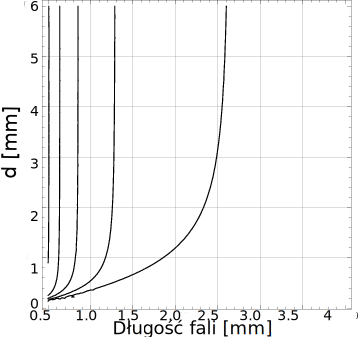
\includegraphics{images/antenaThz/d_lambda.png}
\end{figure}

Wielosc galezi wynika z faktu, ze dla krotszych dlugosci fali rozpatrywany podklad ma charakter wielomodowy. Pojedyncze rozwiazanie powyzej dlugosci fali rownej 3mm, wskazuje nam poczatek zakresu jednomodowego.

\begin{figure}
\includegraphics{images/antenaThz/ro_consrc_radial_antena.png}
\end{figure}

Dla weryfikacji mozliwosci dzialania zaprojektowanych falowodow, przeprowadzono symulacje FDTD we wspolrzednych cylindryczncych. Symulacje potwierdzily mozliwosc wykorzystanie powyzszych siatek zarowno przy oswietleniu ukladu polaryzacja radialna jak  i liniowa. Ponizej przedstawiony rysunek opisuje sytuacje w ktorej struktura z GaAs o rozmiarach 10x10mm pokryta siatka dyfrakcyjna o okresie 538 um i otworach 250um (wspolczynnik wypelnienia ok. 0.53) zostala oswietlona promieniowaniem o dlugosci fali 2.52 mm. W przypadku prezentowanej symulacji siatka miala grubosc 10um, w kolejnych symulacjach potwierdzono jednak, ze grubosc siatki nie ma kluczowego zanczenia pod warunkiem zapewnienia nie przezroczystosci siatki. Efekt koncentracji pola przy zblizaniu sie do srodka struktury wynika ze zmniejszania sie elementu objetosciowego wraz ze zblizaniem do osi symetrii. 




\section{Transmisja jedno kierunkowa}
\section{Soczewka dyfrakcyjna z transmisją jedno kierunkową}





\chapter{Absorbery elektromagnetyczne o~budowie warstwowej}
\label{roz:pml}
Poniższy rozdział traktuje na temat realizacji nie odbijających warstw absorbcyjnych, opartych o koncepcję PML ( wstępnie zaprezentowaną w kontekście metody FDTD w podrozdziale \ref{art:pml}) przy pomocy struktur warstwowych. Rozdział przechodzi od dokładnego wyprowadzenia UPML zgodnie z optyką transformacyjną, do analizy możliwości przybliżenia warstwy UPML za pomocą metamateriału.


\section{Powłoki antyodbiciowe i absorbery}
\subsection{Warstwa antyrefleksyjna}
\begin{figure}[tb]
	\centering
        \begin{subfigure}{0.42\textwidth}
		\includegraphics[width=\textwidth]{images/pml/antiref.png}
                \caption{}
		\label{fig:antyref}
        \end{subfigure}
        \begin{subfigure}{0.47\textwidth}
                \includegraphics[width=\textwidth]{images/pml/sailsbury.png}
                \caption{}
		\label{fig:sailsburyschem}
        \end{subfigure}
        \caption{(a) Schemat prostej warstwy antyodbiciowej  (b) Płytka absorbująca Salisburego}
\end{figure}



\begin{figure}[tb]
	\centering
	\includegraphics[width=\textwidth]{images/antyref.jpg}
	\caption{Zależność współczynnika odbicia od współczynnika załamania warstwy antyrefleksyjnej dla warstwy o grubości $d=\frac{\lambda_0}{4 n_1}$ umieszczonej pomiędzy powietrzem o $n_0=1$, a materiałem o współczynniku załamania $n_2=1.5$}
	\label{fig:antyref-result}
\end{figure}


Działanie prostych absorberów elektromagnetycznych jest analogiczne do warstwy antyodbiciowej. Rozważmy   warstwę antyodbiciową przedstawioną na rysunku \ref{fig:antyref}. Na granicy powietrza i dielektryka o współczynniku załamania $n_2$ wprowadziliśmy inny dielektryk o współczynniku załamania $n_1$, takim że $1<n_1<n_2$. Dokładne wartości współczynnika odbicia od obu granic ośrodków możemy obliczyć za pomocą równań Fresnela. Dla prostoty skupmy się na szczególnym przypadku padania normalnego. Natężeniowy współczynnik odbicia od granicy powietrza i ośrodka o współczynniku załamania $n_2$ wynosi:
\begin{equation}
R=\bigg|\frac{1-n_2}{1+n_2}\bigg|^2.
\end{equation}
Jeżeli jednak pomiędzy powietrze i dielektryk wprowadzimy dodatkową warstwę, wtedy natężeniowy współczynnik odbicia od takiego układu wyraża się wzorem
\begin{equation}
R=\Bigg| \frac{r+r' exp(2 i\phi)}{1+r r' exp(2 i\phi)} \Bigg|^2,
\end{equation}
w którym $r$ i $r'$ oznaczają odpowiednie amplitudowe współczynniki odbicia od granicy ośrodków wynikające z wzorów Fresnela:
\begin{equation}
r=\frac{1-n_1}{1+n_1},
\end{equation}
\begin{equation}
r'=\frac{n_1-n_2}{n_1+n_2},
\end{equation}
a $\phi$ oznacza zmianę fazy fali E-M w trakcie propagacji przez dodatkową warstwę $\phi=k_0 d n_1$, gdzie $d$ to grubość warstwy, $k_0$ to długość wektora falowego w próżni, a $k_y$ to długość wektora falowego w kierunku równoległym do granicy warstw.

 W ten sposób uzyskaliśmy układ dla którego współczynnik odbicia jest mniejszy niż współczynnik odbicia od materiału, ściśle półprzestrzeni wypełnionej materiałem, o współczynniku załamania $n_2$. Zależność współczynnika odbicia od układu z warstwą antyrefleksyjną w zależności od współczynnika załamania $n_1$ dla $n_2=1.46$ przedstawia wykres na rysunku \ref{fig:antyref-result}. Współczynnik odbicia przyjmuje zerową wartość dla $n_1=\sqrt{n_0 n_2}$.

Podstawowym mechanizmem, wykorzystywanym w konstrukcji warstw antyodbiciowych jest interferencja. Dobranie grubości $d=\frac{\lambda_0}{4 n_1}$, gdzie $\lambda_0$ to długość fali w próżni, prowadzi do destruktywnej interferencji między falami odbitymi od pierwszej i drugiej granicy ośrodków. Prowadząc do $R=0$ dla długości fali $\lambda_0$. Powstałe w ten sposób minimum współczynnika odbicia $R=0$, występuje dla wąskiego zakresu długości fali. Możliwe jest uzyskanie niskiego współczynnika odbicia dla szerokiego zakresu długości fali poprzez dodanie kolejnych warstw, o innej grubości optycznej. Współczynniki załamania w tak zbudowanej strukturze muszą zmieniać się zgodnie z postępem geometrycznym $n_i^2=n_{i-1} \cdot n_{i+1}$, a grubość każdej z warstw musi spełniać warunek $d_i=\frac{\lambda_0}{4 n_i}$  Projektując takie struktury możliwe jest uzyskiwanie powierzchni o wybiórczym, ze względu na częstotliwość, współczynniku odbicia~\cite{monacelli2005infrared}. 

\subsection{Ekran Salisbury'ego}
Również na zasadzie interferencyjnego wygaszenia odbicia, działa prosty absorber przedstawiony na rysunku \ref{fig:sailsburyschem}. Przed zwierciadłem w odległości $d$ znajduje się cienka warstwa metalu. Grubość warstwy $d_m$ musi być porównywalna z grubością naskórkową, aby umożliwić transmisję fal E-M przez tę warstwę. W ten sposób pomiędzy zwierciadłem, a cienką warstwą o grubości $d_m$ powstaje wnęka rezonansowa. Zazwyczaj tłumienie wprowadza się za pomocą urojonej części przenikalności $n_1$, możliwe jest jednak oparcie tłumienia jedynie na stratach związanych z grubą warstwą metalową tworzącą zwierciadło. 

\begin{figure}[tb]
	\centering
	\includegraphics[width=\textwidth]{images/pml/sailsbury-res.png}
	\caption{Zależność natężeniowego współczynnika odbicia od grubości warstwy metalowej $d_m$, dla grubości warstwy o współczynniku załamania $n_2=3.34 + 4.27i$ równiej odpowiednio $d=0.2631\lambda_0$ i $d=0.25\lambda_0$}
	\label{fig:sailsburyres}
\end{figure}

Jako przykład,  wykres na rysunku \ref{fig:sailsburyres}  przedstawia zależność współczynnika odbicia od układu przedstawionego na rysunku \ref{fig:sailsburyschem} dla padającego promieniowania o długości fali $\lambda_0$=633~nm w zależności od $d_m$. Jako współczynnik załamania w cienkiej warstwie metalowej przyjęto $n_2=3.34+4.27i$ co odpowiada własnościom chromu dla rozważanej długości fali~\cite{ordal1983optical}. Dobranie odpowiedniej odległości $d$ i grubości warstwy chromu $d_m$ pozwala na wytworzenie warunków destruktywnej interferencji umożliwiając uzyskanie zerowego współczynnika odbicia. W wyniku odbicia na granicy ośrodków o współczynnikach załamania $n_1$ i $n_2$ wprowadzane jest również przesunięcie fazy. Konieczność skompensowania tego przesunięcia, jak i skończone rozmiary warstwy półprzepuszczalnej $d_m$ powodują, że optymalna grubość materiału o współczynniku załamania $n_1$ nieco odbiegają od $\frac{\lambda_0}{4 n_1}$, co ilustrują wyniki na rysunku \ref{fig:sailsburyres}. 

\subsection{Inne propozycje realizacji absorberów}

Innym podejściem jakie można spotkać w literaturze jest wytworzenie warstw nie odbijających za pomocą cienkiej warstwy ferro- i ferimagnetyków tworzących  statyczną magnetyzację o charakterze periodycznym   \cite{ramprecht2008scattering}. Autorzy prezentują wyniki symulacji dowodzące możliwości uzyskania współczynnika odbicia poniżej -20dB w~zakresie od 1 do 4 GHz, niezależnie od kąta padania. W~ostatnich latach proponowane były również absorbery oparte na rezonatorach SRR~(ang.~split-ring resonator), w których warstwa nieodbijająca jest realizowana poprzez uzyskanie dopasowania impedancyjnego z powietrzem jednocześnie wykorzystują stratność w metamateriale. Omówienie prac wykorzystujących tę technikę  można znaleźć w~artykule~\cite{watts2012metamaterial}.

Imponujące wyniki eksperymentalne pozwalające uzyskać wysoki współczynnik absorpcji w szerokim zakresie spektralnym zostały uzyskane za pomocą lasów nanorurek węglowych \cite{mizuno2009black}. Zaprezentowane przez autorów wyniki eksperymentalne wskazują na współczynnik odbicia mniejszy niż 2\% w zakresie od 200~nm do 20µm.

Możliwa jest również konstrukcja absorberów opartych o wielowarstwy metaliczno-dielektryczne. Tego typu absorbery osiągają współczynnik absorpcji większy niż 80\%, dla całego zakresu długości fali ciała doskonale czarnego o temperaturze 300K~\cite{guo2014impact,corrigan2012broadband}. Autorzy dyskutują w pracy dalsze możliwości zmniejszenia współczynnika odbicia poprzez wprowadzenie dodatkowej porowatej warstwy antyodbiciowej. 

W kolejnych podrozdziałach przedstawiona zostanie inna możliwa do zastosowania koncepcja umożliwiająca uzyskanie warstwy charakteryzującej się niskim współczynnikiem odbicia w szerokim zakresie długości fali i kątów padania. 

\section{Wyprowadzenie UPML~(ang. uniaxial perfectly matched layer)}
\subsection{Definicja problemu}
Rozważania dotyczące PML zacznijmy od przytoczenia ogólnej postaci równania falowego~\cite{barton1989elements}
\begin{equation}
\nabla \cdot ( a \nabla u) = \frac{1}{b} \frac{\partial^2 u}{\partial t^2} = \frac{\ddot{u}}{b},
\label{eq:wave}
\end{equation}
gdzie przez $u(\vec{x},t)$ oznaczono skalarną amplitudę fali, $a=a(\vec{x})$ i~$b=b(\vec{x})$ są parametrami, które opisują ośrodek w~którym propaguje się fala. Dla tak sformułowanego równania, możemy zdefiniować wielkość $c=\sqrt{ab}$ mającą interpretację prędkości fazowej fali opisywanej powyższym równaniem. Równanie (\ref{eq:wave}) jest równaniem różniczkowym drugiego rzędu, które możemy zapisać w~postaci układu dwóch równań z~pierwszą pochodną poprzez wprowadzenie pola $\vec{v}(x,t)$:
\begin{equation}
\frac{\partial u}{\partial t} = b \nabla \cdot \vec{v},
\end{equation}

\begin{equation}
\frac{\partial \vec{v}}{\partial t}= a\nabla u.
\end{equation}
Powyższe dwa równania, możemy zapisać  w~postaci równania wektorowego
\begin{equation}
\frac{\partial \vec{w}}{\partial t}=\frac{\partial}{\partial t} {u \choose \vec{v}} = 
	\begin{pmatrix}
		& b\nabla\cdot \\
	a\nabla & \\
	\end{pmatrix}
{u \choose \vec{v}} = \hat{D}\vec{w},
\label{eq:gen-wave-eq}
\end{equation}
dla liniowego operatora $\hat{D}$ i~$\vec{w}=(u;\vec{v})$ ( dla $\vec{v}$ należącego do przestrzeni trójwymiarowej $\vec{w}$ jest czterowektorem). Kluczową własnością, która decyduje o~tym, że równanie~(\ref{eq:gen-wave-eq}) jest równaniem falowym okazuje się być antyhermitowskość operatora $\hat{D}$\footnote{Macierz nazywamy antyhermitowską wtedy gdy spełnia warunek $A$=-$A^\dag$, gdzie przez $^\dag$ rozumiemy sprzężenie hermitowskie macierzy, równoważne dokonaniu transpozycji i~sprzężenia zespolonego wszystkich elementów macierzy.}. To właśnie z~tej własności wynikają oscylujące rozwiązania równania, oraz spełnienie prawa zachowania energii mające kluczowe znaczenie dla fizyki fal. Każde równanie falowe, zaczynając od równań skalarnych, przez równania Maxwella,  po równanie Schr\"{o}dingera i~równania Lam\'{e}-Naviera~(opisującego fale sprężyste w~ciałach stałych) może zostać przedstawione w~formie $ \frac{\partial  \vec{w}}{\partial t}=\hat{D}\vec{w}$, dla pewnej funkcji falowej $\vec{w}$ i~antyhermitowskiego operatora $\hat{D}$~\cite{johnson2007notes}. W niniejszej pracy skupiamy się na zastosowaniu PML w~elektromagnetyzmie, te same koncepcje mogą być jednak zastosowane do wszystkich wymienianych przypadków.

Załóżmy, że $w(x,t)$ jest rozwiązaniem równania falowego w~nieograniczonej przestrzeni. Interesujące nas zjawiska zachodzą w~okolicy początku układu współrzędnych $x=0$, a obszar symulacji chcemy zakończyć tak, aby absorbował fale propagujące się. W szczególności skupimy się na zakończeniu obszaru symulacji dla dodatniej części osi $x$ (rozważanie dla pozostałych kierunków jest analogiczne). Zakończenie obszaru symulacji przeprowadzimy w~czterech krokach:
\begin{enumerate}
	\item W nieskończonej przestrzeni wykonamy analityczne przedłużenie równania falowego i~rozwiązania do zespolonego konturu $\tilde{x}$.
	\item Dla konturu $\tilde{x}$ nie będącego konturem czysto rzeczywistym, fale propagujące się poza interesującym nas obszarem zmieniane są na fale zanikające bez wprowadzenia odbicia.
	\item W nieograniczonej przestrzeni wykorzystamy optykę transformacyjną,  tak aby wyrazić zespolony $\tilde{x}$ przez rzeczywiste położenie. W nowych współrzędnych otrzymamy rzeczywiste położenia i~materiały których własności są opisywane za pomocą liczb zespolonych.
	\item Zakończymy obszar symulacji w~obliczonym na podstawie zamiany zmiennych materiale w~miejscu, w~którym pole będzie na tyle stłumione, aby zastosowany warunek brzegowy nie miał znaczenia.
\end{enumerate}

Zakładamy dalej, że przestrzeń znajdująca się daleko od interesującego nas obszaru w~okolicach $x=0$, jest jednorodna, liniowa i~nie zmienia się w~zależności od czasu. Dzięki tym założeniom, fala propagująca się musi przyjmować formę superpozycji fal płaskich:
\begin{equation}
	w(\vec{x},t)= \sum_{\vec{k},\omega} W_{\vec{k},\omega} e^{i (k_x x-\omega t)},
	\label{eq:pml-cos}
\end{equation}
gdzie $W_{\vec{k},\omega}$ są jedynie funkcjami położenia, $\omega$ częstością kołową, a $\vec{k}$ wektorem falowym dla fali w~ośrodku izotropowym z~zależnością dyspersyjną $\omega=c k_0$, gdzie $c$ oznacza prędkość fazową. Dla fal propagujących się w~kierunku $+x$ prędkość grupowa $\frac{d \omega}{d k}$ jest dodatnia. Kierunek prędkości fazowej i~grupowej w~ośrodkach jednorodnych są zgodne z~wyjątkiem kilku szczególnych przypadków~\cite{teixeira1998general}. Dlatego dalej założymy, że $k_x$ jest dodatnie. 

\begin{figure}[tb]
	\begin{subfigure}{0.45\textwidth}
		\includegraphics[width=\textwidth]{images/pml/real-x.png}
		\caption{}
	\end{subfigure}
	\begin{subfigure}{0.45\textwidth}
		\includegraphics[width=\textwidth]{images/pml/real-x-wave.png}
		\caption{}
	\end{subfigure}


	\begin{subfigure}{0.45\textwidth}
		\includegraphics[width=\textwidth]{images/pml/complex-x.png}
		\caption{}
		\label{fig:complex-contour}
	\end{subfigure}
	\begin{subfigure}{0.45\textwidth}
		\includegraphics[width=\textwidth]{images/pml/complex-x-wave.png}
		\caption{}
		\label{fig:absorbing-region}
	\end{subfigure}

	\caption{Na rysunkach (a) i~(b) przedstawiono odpowiednio rzeczywiste wartości położenia na zespolonej płaszczyźnie $\tilde{x}$ i~odpowiadające im rozwiązanie równania falowego. Na rysunku (c) dla arbitralnej  wartości $\textrm{Re}(\tilde{x})>5$ przedstawiono zmieniony kontur wykorzystujący zespolone wartości dla $\tilde{x}$. Odpowiednie dla zmodyfikowanego konturu (c)  rozwiązanie równania falowego przedstawia wykres na rysunku (d).}
	\label{fig:var-transform}
\end{figure}


Kluczowym jest zauważenie, że składniki sumy z wzoru (\ref{eq:pml-cos}) mogą zostać zapisane w~postaci
\begin{equation}
\vec{W}(y,z)e^{i(k\tilde{x}-\omega t)},
\end{equation}
która to jest funkcją analityczną w~$\tilde{x}\in \mathbb{C}$. Oznacza to, że możemy dokonać jej analitycznego przedłużenia dla zespolonych wartości $x$. Falę propagującą, wraz z~czysto rzeczywistym konturem opisującym położenia w~kierunku $x$ przedstawiają wykresy na rysunku \ref{fig:var-transform}a i~\ref{fig:var-transform}b. 

Dla lepszego zrozumienia koncepcji rozważmy teraz zamianę zmiennych dla obszaru $x>x_0$, w taki sposób, że: 
\begin{equation}
\tilde{x}=  
\begin{cases} 
        x, & \mbox{dla } x< x_0 \\ 
        x+0.2x\mbox{ }i, & \mbox{dla } x>x_0 \\
\end{cases}.
\end{equation}
Rozwiązanie zagadnienia propagacji po takim zespolonym konturze dla $x_0=5$ przedstawia wykres na rysunku \ref{fig:complex-contour}. Zauważymy, że dla obszaru, w~którym do rzeczywistej części dodaliśmy liniowo rosnącą część urojoną uzyskujemy falę zanikającą. Ponieważ na wykresie \ref{fig:absorbing-region} rozwiązanie dla $x<x_0$ nie uległo zmianie, a w~obszarze $x>x_0$ obserwujemy falę zanikającą to przestrzeń dla $x>x_0$ wykazuje działanie nieodbijającej warstwy absorpcyjnej.

\subsection{Rozwiązanie problemu za pomocy zamiany zmiennych}

Zgodnie z przedstawionym przykładem rozwinięcie analityczne możemy dla wygody obliczeniowej traktować równoważnie z~zamianą współrzędnych w~omawianym równaniu różniczkowym. Oznaczmy zespoloną zmienną $\tilde{x}(x)=x+if(x)$, traktując od tej pory $x$ zawsze jako rzeczywiste położenie. Taka zamiana współrzędnych wymaga od nas zamiany każdego różniczkowania po zdeformowanym konturze $\partial \tilde{x} = (1+i\frac{df}{dx}) \partial x$. Ponieważ założyliśmy, że nasze równanie różniczkowe jest niezależne od x (przynajmniej dla dużych x, gdzie $f(x)\ne0$; wynika to bezpośrednio z~założenia jednorodności liniowości i~niezależności od czasu) nie musimy uwzględniać żadnych dodatkowych wyrazów. Jak wykażemy w~kolejnych akapitach wygodnie jest wybrać $\frac{df}{dx}=\frac{\sigma_x}{\omega}$ i~ostatecznie zapisać wymaganą zamianę zmiennych jako:
\begin{equation}
	\frac{\partial}{\partial \tilde{x}} \to \frac{1} {1+i \frac{\sigma_x(x)}{\omega}} \frac{\partial}{\partial x}.
	\label{eq:pml-variable-change}
\end{equation}

W obszarach PML, gdzie $\sigma_x\ne0$, oscylujące rozwiązania równania falowego przyjmują postać fal eksponencjalnie zanikających. Poza PML ( $\sigma_x=0$) rozwiązywane równanie pozostaje niezmienione: nie występują odbicia ponieważ jest to analityczne rozwinięcie pierwotnego rozwiązania i~w obszarach gdzie $\tilde{x}=x$ rozwiązanie nie może się zmienić.

Po wykonaniu podstawienia (\ref{eq:pml-variable-change}), rozwiązania równania falowego w~obszarze PML przyjmują postać:
\begin{equation}
e^{ikx}\textrm{exp}\Big(-\frac{k}{\omega}\int^x \sigma_x(x')dx'\Big).
\end{equation}
Warto zauważyć, że pojawiający się wykładnik potęgi $\frac{k}{\omega}$ dla materiałów bezdyspersyjnych jest stały i~równy odwrotności prędkości fazowej. W ten sposób uzasadniliśmy zaproponowany wybór $\frac{df}{dx}=\frac{\sigma_x}{\omega}$, dzięki któremu otrzymujemy niezależność współczynnika tłumienia od częstotliwości promieniowania E-M. 

\subsection{Wynik przeprowadzonej analizy}
Zgodnie z~przedstawionym wyprowadzeniem możemy zastosować dowolnie mały obszar PML, ponieważ nie ma żadnego ograniczenia na wartości $\sigma_x$. W praktyce numerycznej, ze względu na zastosowaną dyskretyzację gwałtowne zmiany $\sigma_x$ prowadzą do powstania ,,odbić numerycznych''. Z tego powodu $\sigma_x$ zazwyczaj ma postać funkcji kwadratowej lub sześciennej narastającej od zera do wartości maksymalnej na obszarze większym od połowy długości fali promieniowania występującego w~symulacji~\cite{johnson2008notes}.

W przypadku równań Maxwella każda zamiana współrzędnych może zostać wyrażona przez równania Maxwella we współrzędnych kartezjańskich ze zmienionymi materiałami~\cite{ward1996refraction}. Zamiana współrzędnych jest równoważna zmianie przenikalności elektrycznej $\varepsilon$ i~magnetycznej µ, w~ogólności na absorbujące ośrodki anizotropowe. W dalszej części rozdziału zakładać będziemy, że warstwa PML jest usytuowana tak, że jej powierzchnia zewnętrzna jest prostopadła do osi $z$.

W przypadku trójwymiarowych równań Maxwella dla ośrodka opisywanego za pomocą tensorów $\hat{\varepsilon}$ i~$\hat{\mu}$ 
\begin{equation}
\hat{\varepsilon}=
\begin{bmatrix}
\varepsilon_x & 0 & 0 \\
0 &\varepsilon_y & 0 \\
0 & 0  & \varepsilon_z  \\
\end{bmatrix}
, \hat{\mu}=
\begin{bmatrix}
\mu_x & 0 & 0 \\
0 &\mu_y & 0 \\
0 & 0  & \mu_z  \\
\end{bmatrix}
\end{equation}
warstwą PML może być materiał charakteryzujący się przenikalnością elektryczną i~magnetyczną opisywaną tensorami:
\begin{equation}
\hat{\varepsilon}_{\textrm{PML}}=
\begin{bmatrix}
s \cdot \varepsilon_x & 0 & 0 \\
0 &s \cdot \varepsilon_y & 0 \\
0 & 0  & \frac{ \varepsilon_z}{s}  \\
\end{bmatrix}
, \hat{\mu}_{\textrm{PML}}=
\begin{bmatrix}
s \cdot \mu_x & 0 & 0 \\
0 & s \cdot \mu_y & 0 \\
0 & 0  & \frac{\mu_z}{s}  \\
\end{bmatrix},
\label{eq:general-pml-form}
\end{equation}
gdzie $s$ jest dowolną liczbą zespoloną~\cite{sacks1995perfectly}, której część odpowiedzialna za tłumienie jest równoznaczna liniowemu współczynnikowi deformacji konturu zmiennych przestrzennych w~część urojoną.



\section{PML ze struktury warstwowej~\cite{ania2015}}
\begin{figure}[tb]
	\includegraphics[width=\textwidth]{images/pml/oqe_schemat.png}
	\caption{Schematyczne przedstawienie analizowanej struktury warstwowej i przybliżanego przy pomocy modelu ośrodka efektywnego ośrodka PML}
	\label{fig:pml-multilay-schem}
\end{figure}

Porównując ogólną postać PML podaną w równaniu (\ref{eq:general-pml-form}) z modelem ośrodka efektywnego przedstawionym w podrozdziale \ref{subart:effmedium} można zaproponować przybliżenie ośrodka typu PML przy pomocy struktury warstwowej o odpowiednich właściwościach efektywnych. W szczególności dla uproszczenia analizy skupimy się na polaryzacji TM, dla której istotnymi składowymi tensorów opisujących własności materiałowe są:$\varepsilon_x$,$\mu_y$i $\varepsilon_z$. Ze względu na ograniczenia używanego modelu ośrodka efektywnego, zgodnie ze schmatem na rysunku \ref{fig:pml-multilay-schem} $\varepsilon_x=\varepsilon_y$, oraz $\mu_x=\mu_y$. Ponownie odwołując się do granicy między ośrodkami przedstawione na rysunku \ref{fig:pml-multilay-schem} warunki dla których wielowarstwa będzie efektywnie spełniać rolę PML przedstawiają się następująco:
\begin{equation}
	f\cdot \varepsilon_{w1} + (1-f)\cdot \varepsilon_{w2} = s \cdot \varepsilon_1,
	\label{eq:oqe4}
\end{equation}

\begin{equation}
	[f\cdot \varepsilon_{w1}^{-1}+(1-f)\varepsilon_{w2}^{-1}]^-1=s^{-1}\cdot \varepsilon_1,
	\label{eq:oqe5}
\end{equation}

\begin{equation}
	f\cdot \mu_{w1} + (1-f)\cdot \mu_{w2} = s \cdot \mu_1,
	\label{eq:oqe6}
\end{equation}
gdzie przez $f$ oznaczony został współczynnik wypełnienia, równy ułamkowi przestrzeni wielowarstwy zajmowanemu przez materiał $w1$. Odpowiednie warunki dla polaryzacji TE to:
\begin{equation}
	\varepsilon_{w1}=\rho \frac{\varepsilon_1 \cdot s}{f\cdot \rho + (1 -f) },
	\label{eq:te-eps1}
\end{equation}

\begin{equation}
	\varepsilon_{w2}=\frac{\varepsilon_1 \cdot s}{f\cdot \rho + (1-f)},
	\label{eq:te-eps2}
\end{equation}
gdzie
\begin{equation}
	\rho = 1+\frac{s^2-1 \pm \sqrt{(s^2-1)(s^2-(2f-1)^1)}}{2f(1-f)}.
	\label{eq:te-rho}
\end{equation}

\begin{figure}[tb]
	\includegraphics[width=\textwidth]{images/pml/oqe_materials.png}
	\caption{Zależność przenikalności elektrycznej materiałów tworzących UPML (w lewej kolumnie $\varepsilon_{w1}$, w prawej $\varepsilon_{w2}$) w funkcji współczynnika wypełnienia i urojonej części parametru $s$ (założono $\textrm{Re(s)=1}$. Górny wiersz na wykresach (a) i (b) prezentuje zależności części rzeczywistych, dolny na wykresach (c) i (d) części urojonych przenikalności elektrycznych. Ujemne wartości $\varepsilon$ na wykresach (c) i (d) odpowiadają materiałom ze wzmocnieniem optycznym. }
	\label{fig:upml-eps-s-f}
\end{figure}

Wykresy na rysunku \ref{fig:upml-eps-s-f} prezentują wyniki obliczonych (\ref{eq:te-eps1}) i (\ref{eq:te-eps2}) jako funkcję współczynnika wypełnienia $f$ i parametru $s$, dla którego przyjęto $s=1+\alpha i$. Używamy rozwiązań dla (\ref{eq:te-rho}) z $|\rho|>1$. Podobne wyrażenia jak (\ref{eq:oqe4}) i (\ref{oqe5}) można wypisać i rozwiązać dla $\mu_{w1}$ i $\mu_{s2}$. W przypadku gdy $\varepsilon_1=\mu_1$ otrzymujemy $\varepsilon_{w1}=\mu_{w1}$ i $\varepsilon_{w2}=\mu_{w2}$. 

Zależność współczynnika odbicia od kąta padania, oraz grubości komórki elementarnej wielowarstwy przedstawia wykres na rysunku \ref{fig:oqe3}. Ze względu na umieszczenie idealnego przewodnika za wielowarstwą współczynnik odbicia łączy w sobie część odbijaną od wielowarstwy, jak i transmitowaną przez wielowarstwę i odbijaną od zwierciadła z PEC. Analizując wykres \ref{fig:oqe3} możemy zauważyć, że wraz ze wzrostem $\frac{a}{\lambda}$ zmniejsza się współczynnik odbicia fal propagujących się $\frac{k_x}{k_0}<1$. Wynika to z faktu jednoczesnego zwiększania grubości warstwy pochłaniającej, więc jest przedewszystkim związane ze zmniejszeniem transmisji przez wielowarstwę. W przypadku fal ewanescętnych $\frac{k_x}{k_0}>1$ obserwujemy wzrost współczynnika odbicia. Można to interpretować jako odbicie od pierwszej warstwy wynikające z niespełnienia warunków homogenizacji (przybliżenie ośrodka efektywnego zakłada $\frac{a}{\lambda} \to 0$) przez strukturę. Dlatego wzrost jest większy dla większej części urojonej współczynnika $s$, skutkującej większą różnicą współczynników załamania na granicy pierwszej warstwy i powietrza.

\begin{figure}[tb]
	\includegraphics[width=\textwidth]{images/pml/fig3.png}
	\caption{Zależność natężeniowego współczynnika odbicia od kąta padania i okresu wielowarstwy dla struktury zgodniej ze schmatem na rysunuku \ref{fig:pml-multilay-schem}, dla $N=5$ par warstw, przy współczynniku wypełnienia $f=0.6$. Wysunek po lewej (a) przedstawia wyniki dla $s=1+0.5i$, wykres po prawej przedstawia wyniki dla $s=1+5i$.}
	\label{fig:oqe3}
\end{figure}

Przedstawione wyniki możliwe są do osiągnięcia przy pomocy materiałów wykazujących szczególne własności elektryczne i magnetyczne, w szczególności obliczenia zakładały zespoloną przenikalność magnetyczną, oraz zysk optyczny. Dla $s=1+5i$ możliwe jest uzyskanie warstwy PML o całkowitej grubości $5\cdot a \approx \frac{\lambda}{20}$ wykazującej natężeniowy współczynnik odbicia ok -30dB dla szerokiego zakresu kątów padających fal płaskich.

W przypadku oświetlenia wielowarstwy przy pomocy polaryzacji TM jeden ze współczynników przenikalności magnetycznej może zostać ustalony w sposób arbitralny. W szczególności możemy więc założyć $\mu_{w2}=1$, ponieważ większość materiałów spotykanych w przyrodzie charakteryzuje się taką wartością dla częstotliwości optycznych. Drugą przenikalność magentyczną możemy wyznaczyć przy pomocy wzoru \ref{eq:oqe6}. Część rzeczywista $\textrm{Re}(\mu_{w1})=1$, a zależność części urojonej $\textrm{Im}(\mu_{w1})$ od części urojonej współczynnika $s$, oraz współczynnika wypełnienia przedstawia wykres \ref{fig:im-mu1}. Na podstawie przywołanego wykresu możemy zauważyć, że wysoki współczynnik wypełnienia, oraz wykorzystanie małej części urojonej $s$ skutkują małymi wartościami $\textrm{Im}(\mu_{w1})$, jest to dla nas istotne ponieważ korzystając z realnych materiałów będziemy zmuszeni przybliżyć te wartość przez $0$.

\begin{SCfigure}
	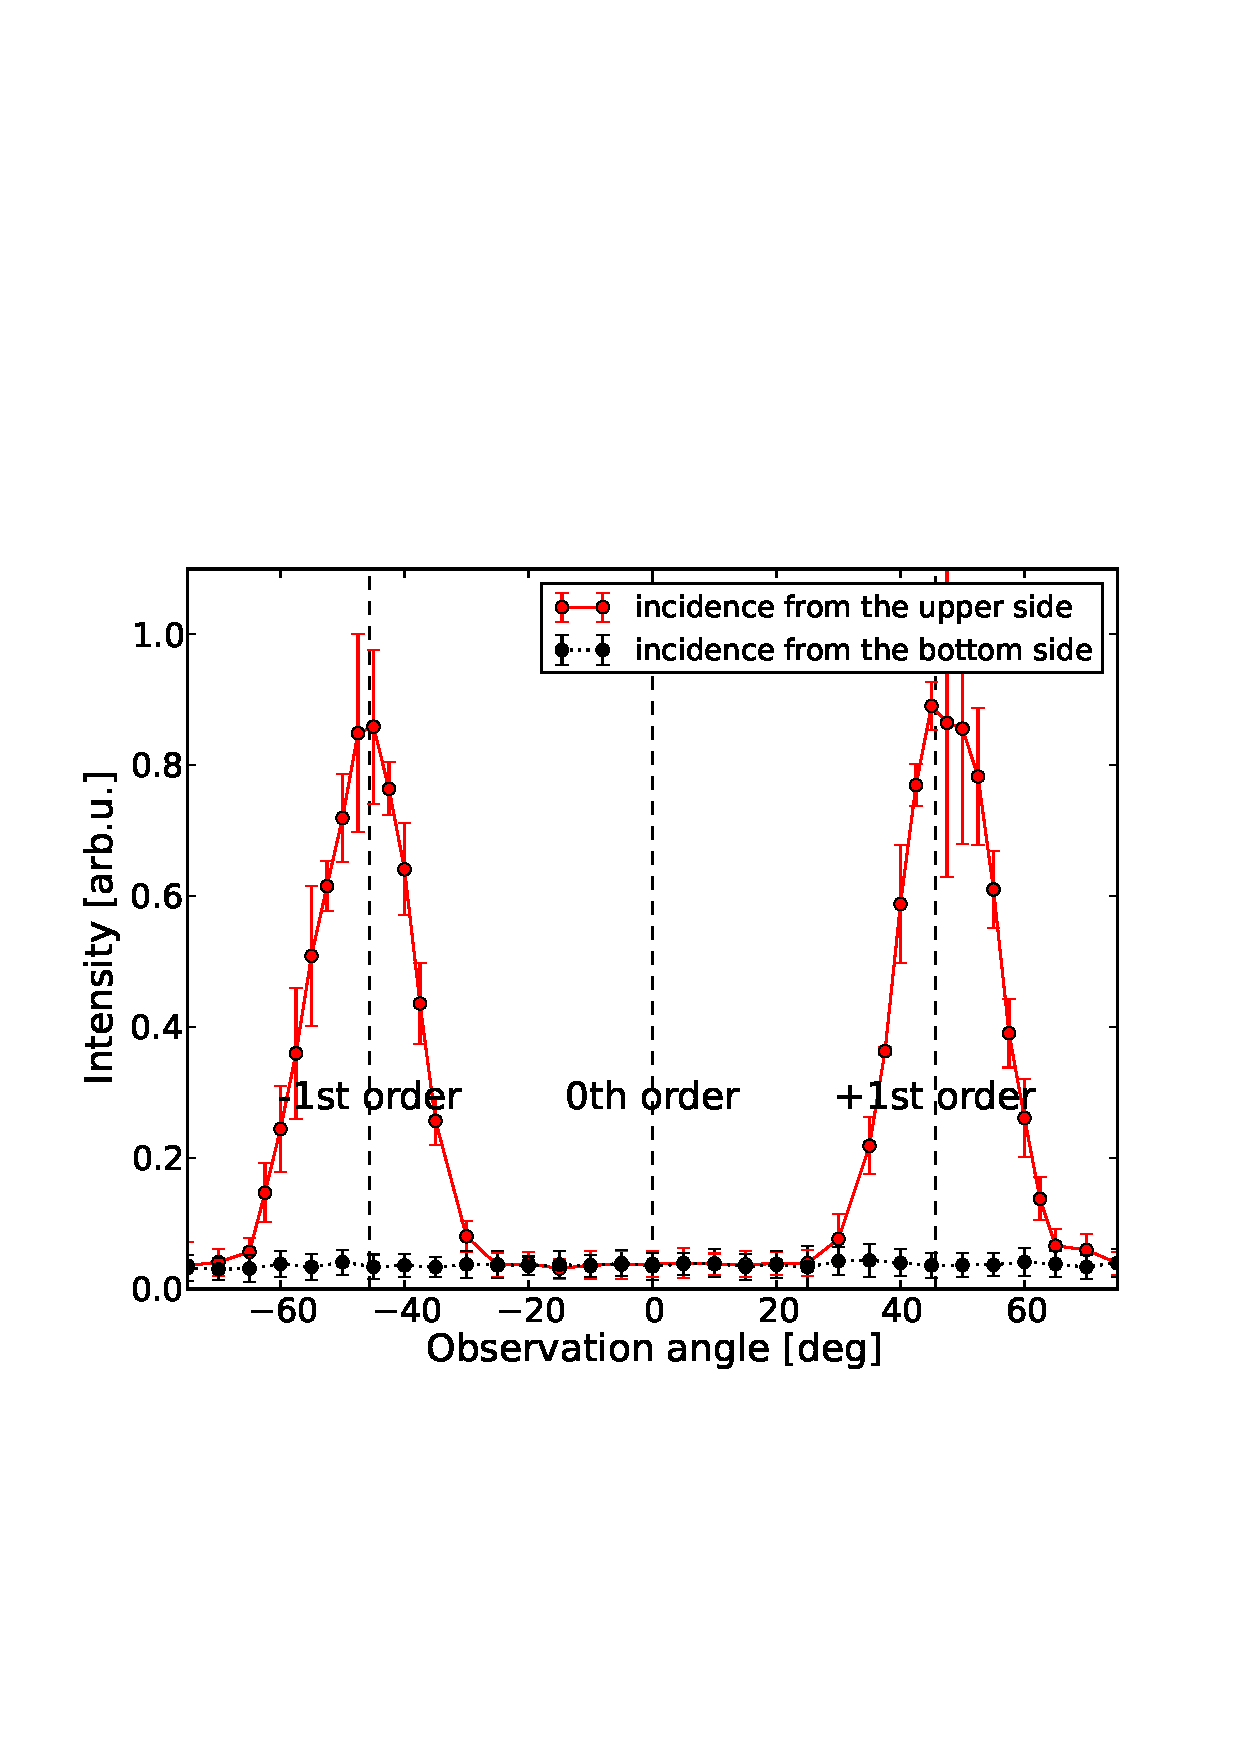
\includegraphics[width=0.6\textwidth]{images/pml/fig4.png}
	\caption{Zależność części urojonej przenikalności magnetycznej jednego z materiałów $\mu_{w1}$, od części urojonej współczynnika $s$ i współczynnika wypełnienia $f$ w przypadku gdy założono $\mu_{w2}=1$}
	\label{fig:im-mu1}
\end{SCfigure}


W przypadku zastosowania nie numerycznego należy zaniedbać własności magnetyczne materiałów $\mu=1$, oraz zysk optyczny $\textrm{Im}(\varepsilon)\ge0$. Wyniki dla obu polarizacji po zasotosowaniu się do wymienionych przybliżeń przedstawiają wykresy na rysunku \ref{fig:pml-real-ref}. Zaproponowany absorber skład się z materiału stratnego, oraz warstw charakteryzujących się przenikalnością elektryczną mniejszą od 1. Przedstawione wyniki obliczeń wskazują, że w wyniku poczynionych założeń efektywność pracy wielowarstwy jako struktury PML znacznie różni się w zależności od polaryzacji. W przeciwieństwie do obliczeń dla wielowarstw odpowiadających PML, narzucone wartunki prowadzą do mniejszej wartości współczynnika odbicia dla polaryzacji TE. Wysokie współczynniki odbicia, uniemożliwiające zastosowanie wielowarstwy,  pojawiają się jednak jedynie dla kątów padania bliskich $90^{\circ}$, co jest charakterystyczne dla UPML.

\begin{figure}[tb]
	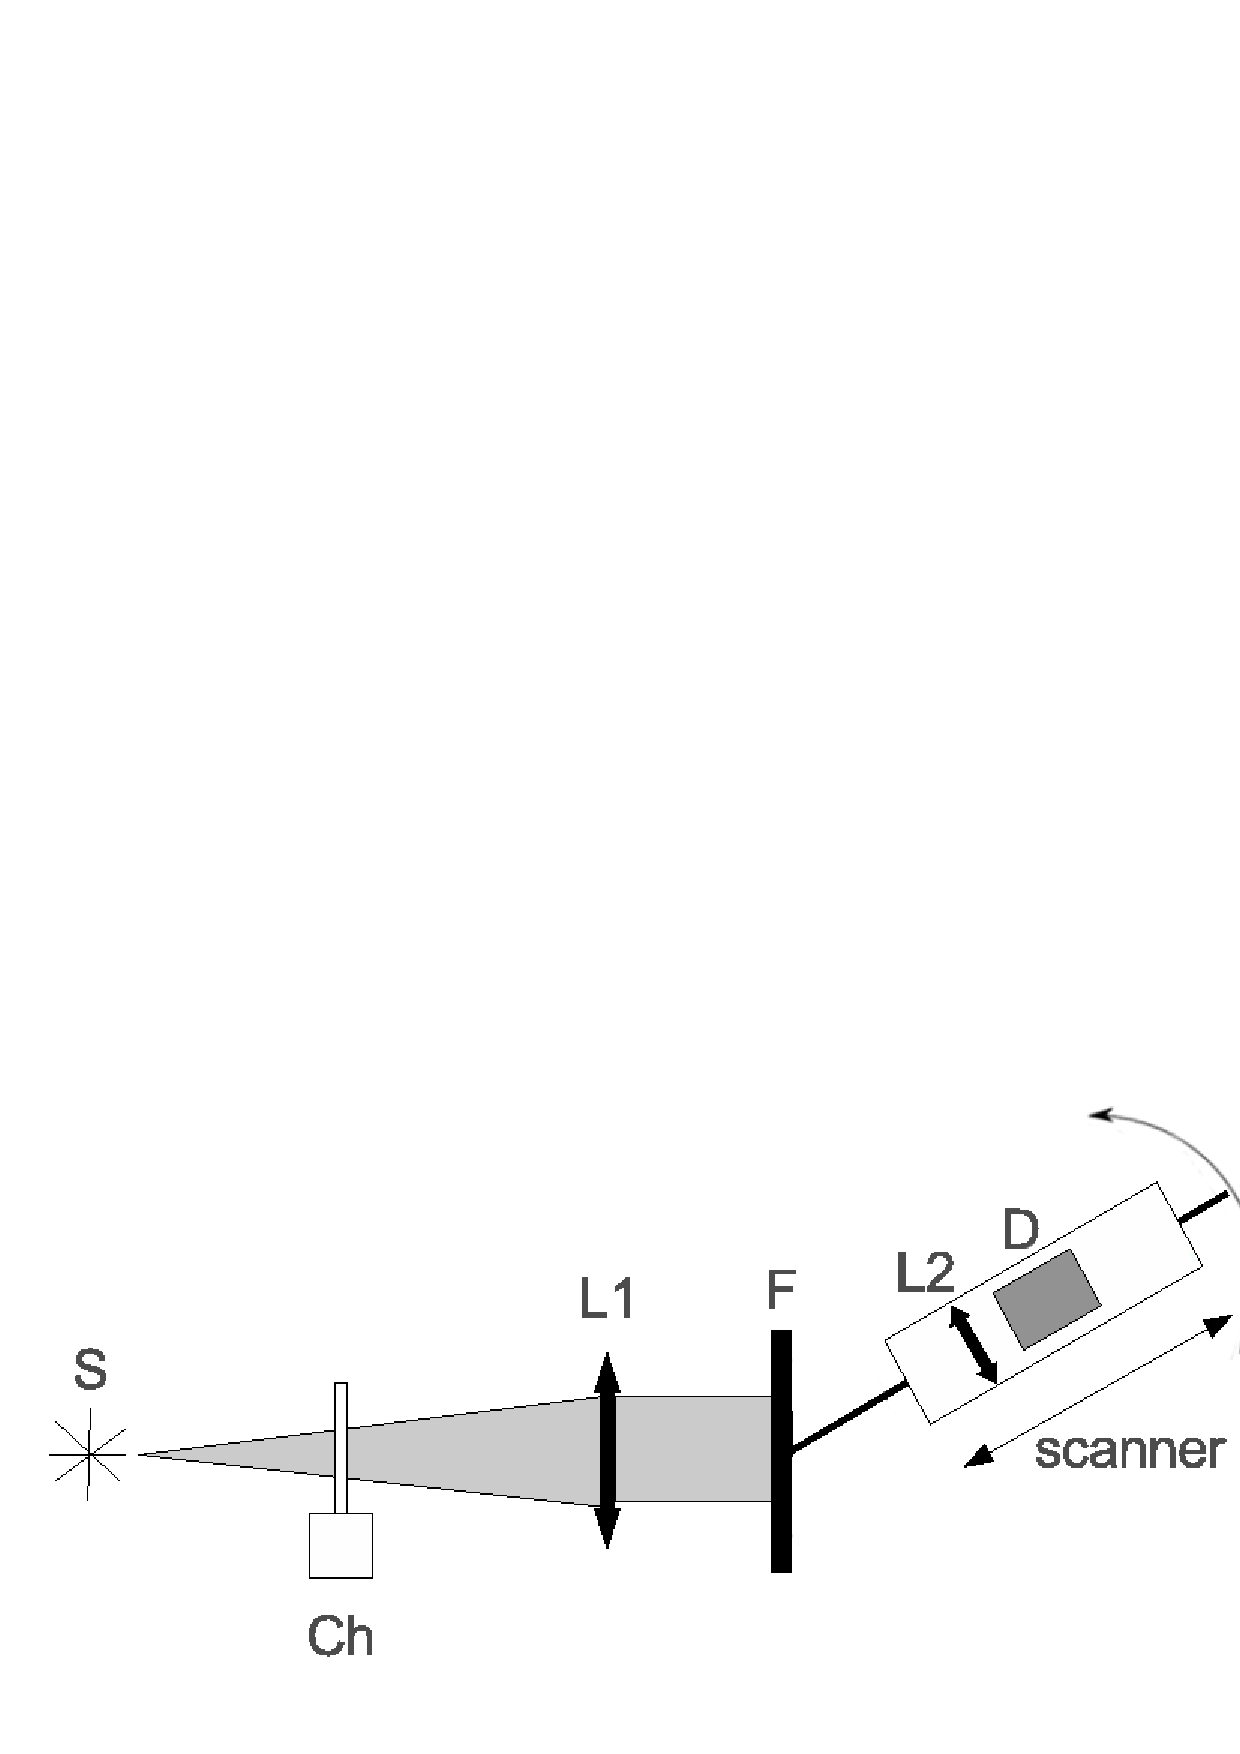
\includegraphics[width=\textwidth]{images/pml/fig5.png}
	\caption{Zależność natężeniowego współczynnika odbicia $R$, od kąta padania i grubości warstw dla wielowarstwy składającej się z $N=5$ okresów, dla $s=1+5i$ i $f=0.6$. Spełniając założenie, że $\mu_{w2}=1$ (a,c), oraz $\mu_{w1}=\mu_{w2}=1$, $\textrm{Im}(\varepsilon_1)\ge 0 $ i $\textrm{Im}(\varepsilon_2)\ge 0 $ (b,d). Wyniki dla polaryzacji TM (a,b) oraz TE (c,d). Przenikalnośc elektryczna $\varepsilon_{w1}=1.474+1.017i$.}
	\label{fig:pml-real-ref}
\end{figure}


Na podstawie przeprowadzonej dyskusji, można wysunąć prostą regułę jaką należy posługiwać się w celu doboru materiałów do budowy wielowarstwy efektywnie przypominającej UPML graniczący z powietrzem. Kluczowym elementem jest wykorzystanie materiału którego część rzeczywista przenikalności elektrycznej znajduje się w zakresie od 0 do 1. Przeprowadzone obliczenia wskazują również, że materiał ten powinien być możliwe bezstratny. Druga wykorzystywana substancja powinna posiadać część rzeczywistą przenikalności elektrycznej większą od 1, oraz wykazywać stratność. 

W ogólności w szerokich zakresach spektralnych większość materiałów charakteryzuj się $\textrm{Re}(\varepsilon) > 1$, wyjątkami są zakresy długości fali w okolicach rezonansów dyspersyjnych (patrz. \ref{subart:lorenz-drude}). Możliwe jest również uzyskanie zaprojektowanych własności $\varepsilon$ w metamateriałach np. w strukturach typu fishnet~\cite{valentine2008three}. Przykładem pary materiałów, które możemy zastosować w realizacji UPML przy pomocy wielowarstwy są $SiO_2$ i $NaCl$ dla długości fali w okolicach 8~$\mu$m. Przenikalności elektryczne zaproponowanych materiałów przedstawiają wykresy na rysnuku \ref{fig:nacl-sio2-mat}. Rolę materiału o przenikalności elektrycznej $\varepsilon \in (0,1)$, spełnia w tym obszarze $SiO_2$, ponieważ dla długości fali $9.5$~$\mu$m występuje dla tego materiału rezonans również efektywna część urojona wielowarstwy wynika głównie z własności $SiO_2$. 

\begin{figure}[tb]
	\begin{subfigure}{0.45\textwidth}
		\includegraphics[width=\textwidth]{images/pml/nacl.png}
		\caption{}
	\end{subfigure}
	\begin{subfigure}{0.45\textwidth}
		\includegraphics[width=\textwidth]{images/pml/sio2.png}	
		\caption{}
	\end{subfigure}
	\caption{Wartości przenikalności elektrycznej w zakresie od 7 do 10~$\mu$m dla (a) $NaCl$~\cite{li1976refractive}, (b) $SiO_2$~\cite{Kischkat:12}}
	\label{fig:nacl-sio2-mat}
\end{figure}

Efektywne własności stosu złożonego z naprzemiennych warstw $NaCl$ i $SiO_2$ o współczynniku wypełnienia drugim materiałem $f=0.56$, dla których przyjęto zmierzone eksperymentalnie wartości $\varepsilon$ przedstawia wykres na rysunku \ref{fig:eff-pml-real}. Zgodnie z (\ref{eq:general-pml-form}) warstwa opisywana struktura przypominająca PML powinna charateryzować się $\frac{1}{\varepsilon_x}=\varepsilon_z$, dlatego na wykresie zaznaczono również $\frac{1}{\varepsilon_x}$. Na podstawie wykresu \ref{fig:eff-pml-real} wielowarstwa powinna więc charakteryzować się najniższym współczynnikiem odbicia dla długości fali z zakresu 8-8.2~$\mu$m. Wartości natężeniowych współczynników transmisji i odbicia w zależności od liczby par warstw $N$ oraz długości fali przedstawia wykres na rysunku \ref{fig:oqe-trans-refl}.

\begin{SCfigure}
	\includegraphics[width=0.6\textwidth]{images/pml/effepsilon-nacl-sio2.png}
	\caption{Współczynniki efektywne wielowarstwy zbudowanej z $SiO_2$ i $NaCl$, o współczynniku wypełnienia przez $SiO_2$ równym $f=0.56$, dla eksperymentalnych wartości $\varepsilon$.}
	\label{fig:eff-pml-real}
\end{SCfigure}

Bazując na zaprojektowanej wielowarstwie można zaproponować jej realizację w geometrii cylindrycznej. W tym przypadku jakość nieodbijającej warstwy absorbcyjnej możemy ocenić na podstawie symulacji, w których wewnątrz struktury typu core-shell zamknięty zostanie walec z idealnego przewodnika. Rozkład gęstości energii pola E-M dla struktury typu core-shell odpowiadającą rozważanej wielowarstwie, oświetlonoą falą monochromatyczną dla polaryzacji TM~i~TE przedstawia rysunek 

\begin{figure}[tb]
	\centering
	\includegraphics[width=0.6\textwidth]{images/pml/oqe_trans_refl.png}
	\caption{Współczynnik transmisji (linia ciągła) i odbicia (linia przerywana) dla wielowarstwy złożonej z $SiO_2$/$NaCl$ zaprojekowanej dla oświetlenia długością fali 8~$\mu$m, dla której współczynniki załamania $n_{\textrm{SiO}_2}=0.41+0.32i$, $n_{\textrm{NaCl}}=1.51$. Współczynnik wypełnienia struktury przez $SiO_2$ wynosi $f=0.56$, $a=200nm$. Rozważone zostały stosy o $N=10,100,400$.}
	\label{fig:oqe-trans-refl}
\end{figure}

\begin{figure}[tb]
	\includegraphics[width=\textwidth]{images/pml/oqe_coreshell.png}
	\caption{Wyniki symulacji we współrzędnych cylindrycznych dla polaryzacji (a) TE i (b) TM. Struktura typu core-shell oświetlona jest z dołu, na rysunku (a) zamieszczono wzorzec długości fali.}
\end{figure}





Każdy element układu optycznego możemy wyrazić jako układ filtrujący częstotliwość i częstości przestrzenne oświetlającego ten układ źródła. Poniższy rozdział poświęcony jest modelowaniu działania wielowarstw metaliczno-dielektrynych wykorzystywanych do  budowy elementów optycznych o zaprojektowanych własnościach filtrowania częstości przestrzennych. W przeciwieństwie do przestrzeni swobodnej, będącej filtrem dolnoprzepustowym, mogą one charakteryzować się również transmisją wysokich częstości przestrzennych, które w przestrzeni swobodnej mają charakter fal ewanescentnych. Wykorzystanie układów tego typu umożliwia konstrukcję elementów optycznych działających poza klasycznym ograniczeniem dyfrakcyjnym.

Złamanie ograniczenia dyfrakcyjnego możliwe jest dzięki zastosowaniu materiałów charakteryzujących się ujemnym załamaniem światła, rozumianym jako załamanie pod kątem skierowanym przeciwnie niż wynikałoby to z Prawa Snelliusa. Materiały takie w odniesieniu do przywołanej klasycznej formuły optyki geometrycznej muszą charakteryzować się ujemnym współczynnikiem załamania światła. Korzystając z elektrodynamiki klasycznej opisywanej równaniami Maxwella wiemy, że współczynnik załamania związany jest z przenikalnością elektryczną i magentyczną ośrodka: $n = \pm \sqrt{ \varepsilon \mu}$. Wybór dodatniej gałęzi pierwiastka jest więc konwencjonalny i musi być dostosowany do sytuacji fizycznej. Ujemna wartość współczynnika załamania światła jest równoważna ze zmianą kierunku prędkości fazowej, której zwrot jest zgodny ze zwrotem wektora falowego. Pierwszą propozycją definicji ośrodków o ujemnym współczyniku załamania była ujemna wartośc iloczynu skalarnego wektora Poyntinga i wektora falowego $\vec{P} \cdot \vec{k} < 0$ podana przez Victora Vesselago \cite{veselago1968electrodynamics}. Ze względu na tę własność materiały takie nazywane są lewoskrętnymi (ang. left-handed) gdyż w stosunku do do iloczynu $\vec{E} \times \vec{H}$ nie ma zastosowania reguła prawej dłoni, a przeciwna - lewej.

Materiały lewoskrętne muszą charakteryzować się ujemnymi wartościami $\varepsilon$ i $\mu$ dla tego samego zakresu częstotliwości. Materiały takie nie były do tej pory obserwowane w przyrodzie, eksperymentalnie dowiedziono jednak możliwość sztucznego wytworzenia metamateriałów o takich własnościach\cite{PhysRevLett.84.4184} przy pomocy SSR(ang split-ring resonator). 

Język używany do opisu działania analizowanych struktur warstwowych wywodzi się z Optyki Fourierowskiej w której podstawowym pojęciem są układy LSI (ang. Linear shift-invariant systems). Opisywane struktury spełniają warunki tego typu układów - nie wykazują własności nieliniowych, oraz są niezmiennicze ze względu na przesunięcia. Wykorzystanie formalizmu Optyki Fourierowskiej umożliwia analityczną ocenę wyników symulacji numerycznych, oraz wprawdza spójny zestaw pojęć wykorzystywanych do opisu rozważanych układów. Dokładniejsze omówienie podstawowych pojęć związanych z układami LSI znajduje się w rozdziale \ref{art:lsi}.



\section{Wlasnosci materialowe w zakresie widzialnym}
Zjawiska omawiane w tym rozdziale są ściśle związane z wykorzystaniem zakresów długości fali elektormagnetycznej dla których stosowane materiały wykazują specyficzne własności. Na wykresie \ref{ag-permittivity} przedstawiono zależność zespolonego współczynnika przenikalności dielektrycznej od długości fali, na podstawie danych z [\ref{palik}]

\begin{figure}
\label{ag-permittivity}
\end{figure} 

\subsection{Model Lorenza}
Własności materiałowe w tym modelu opisywane są przez


\section{wielowarstwy z bezdyfrkacycyjną propagacja swiatla}
\section{nadrozdzielczy pryzmat}
\section{analiza chropowatosci}
\section{bardziej zlozone struktury skladane wielowarstw}

\bibliographystyle{plain}
\bibliography{bibliografia}




\chapter{Podsumowanie}
Poniższa praca jest wynikiem kilku lat studiów doktoranckich autora, w~trakcie których prowadził on symulacje, których celem było projektowanie i~optymalizacja struktur o~rozmiarach podfalowych. Podstawowym narzędziem wykorzystywaną przez autora były obliczenia numeryczne metodą FDTD przy pomocy aplikacji meep\cite{OskooiRo10} na komputerach dużej mocy udostępnianych w~ramach Interdyscyplinarnego Centrum Modelowania Matematycznego i~Komputerowego UW, oraz infrastruktury PLgrid. Pomimo zastosowania podobnych metod obliczeniowych przedstawione w~różnych rozdziałach układy kierowane były dla różnych zakresów długości fali.

Zaczynając od układów do jednokierunkowej transmisji i~skupiania wiązki światła dla zakresu THz (długości fali ok.~3~cm), które zostały przedstawione w~rozdziale \ref{chap:thz}. Prace te koncentrowały się na projektowaniu i~optymalizacji układów, które podlegały późniejszej weryfikacji eksperymentalnej. Wyniki tych prac wskazały na możliwość uzyskania jednokierunkowej transmisji, zgodnej z~twierdzeniem o~wzajemności, w~-1~i~+1 rzędzie dyfrakcyjnym.

Przez zakres podczerwony, dla którego w~rozdziale \ref{roz:pml} przedstawiono prace numeryczne zawierające propozycję realizacji nie odbijającej warstwy pochłaniającej przy pomocy układów warstwowych. Całość projektu przedstawia analizę opartą na wyidealizowanych~(nieistniejących fizycznie materiałach), przez serię przybliżeń, aż do symulacji opartych o~własności materiałowe zaczerpnięte z~prac eksperymentalnych.

W przedostatnim,  rozdziale \ref{art:nondiff}  omówione zostały struktury fotoniczne dla światła widzialnego~(długości fali rzędu kilkuset~nanometrów). Przedstawiono, w~szerokim kontekście literaturowym, wkład autora w~badania dotyczące układów opartych o~wielowarstwy metaliczno-dielektryczne przeznaczone do obrazowania, rzutowania i~koncentracji wiązek promieniowana E-M o~rozmiarach podfalowych.





\printnomenclature

\addcontentsline{toc}{chapter}{Bibliografia}
%\bibliographystyle{abbrvnat}
\bibliographystyle{osa}
\bibliography{bibliografia}

\addcontentsline{toc}{chapter}{Spis ilustracji}
%\listoffigures
\end{document}
